\documentclass[11pt,a4paper]{article}
\usepackage[T1]{fontenc}
\usepackage[utf8]{inputenc}
\usepackage{lmodern,microtype,amsmath,amssymb,amsthm,mathtools,bm}
\usepackage[margin=26mm]{geometry}
\usepackage{graphicx,booktabs,array,xcolor,enumitem}
\usepackage[colorlinks=true,linkcolor=violet,citecolor=violet,urlcolor=violet,breaklinks=true]{hyperref}
\hypersetup{pdftitle={Extrinsic curvature bias in Sinkhorn metrics},pdfauthor={Anonymous},pdfsubject={Fixed-cost continuous-density limit and curvature correction}}
\usepackage{fancyhdr}
\pagestyle{fancy}\fancyhf{}\fancyhead[L]{\small Sinkhorn metrics and extrinsic curvature}\fancyhead[R]{\small Preprint}\fancyfoot[C]{\thepage}
\setlength{\headheight}{14pt}
\setlength{\emergencystretch}{2em}
\newtheorem{theorem}{Theorem}[section]
\newtheorem{lemma}[theorem]{Lemma}
\newtheorem{proposition}[theorem]{Proposition}
\newtheorem{corollary}[theorem]{Corollary}
\theoremstyle{definition}\newtheorem{definition}[theorem]{Definition}
\theoremstyle{remark}\newtheorem{remark}[theorem]{Remark}
\newcommand{\eps}{\varepsilon}
\newcommand{\dd}{\,\mathrm d}
\newcommand{\R}{\mathbb R}
\newcommand{\Id}{\mathrm{Id}}
\newcommand{\diver}{\operatorname{div}}
\newcommand{\tr}{\operatorname{tr}}
\newcommand{\KL}{\operatorname{KL}}
\newcommand{\OT}{\operatorname{OT}}
\newcommand{\II}{\mathrm{II}}
\newcommand{\Ric}{\operatorname{Ric}}
\newcommand{\Scal}{\operatorname{Scal}}
\newcommand{\ip}[2]{\langle #1,#2\rangle_\mu}
\newcommand{\norm}[1]{\lVert #1\rVert}
\newcommand{\M}{\mathcal M}
\newcommand{\SD}{\mathcal S}
\title{Extrinsic curvature bias in the small-regularisation limit of Sinkhorn metrics\\[4pt]\large A fixed-cost continuous-density theorem on closed embedded manifolds}
\author{Anonymous}
\date{4 November 2026 (revised)}
\begin{document}
\maketitle
\begin{abstract}
Let a smooth positive probability density be supported on a compact connected smooth submanifold of Euclidean space without boundary, and fix the ambient squared-distance transport cost. We prove that the Sinkhorn metric operator converges in operator norm on centred $L^2$ to the inverse weighted Laplacian, at rate $O(\eps^{1/2})$ in $L^2$ operator norm and $O(\eps)$ from $H^2$ to $L^2$. For a smooth tangent $h\mu$, with $A\phi=h$ and $A=-\rho^{-1}\diver(\rho\nabla)$, we identify the first correction:
\[
g_{\eps,\mu}(h\mu,h\mu)=\int|\nabla\phi|^2\dd\mu
-\frac{\eps}{4}\int\sum_\alpha|S_\alpha\nabla\phi|^2\dd\mu+O(\eps^2),
\]
where $S_\alpha$ are the shape operators of the embedding. The first bias is therefore nonpositive and depends on the embedding, not only on the intrinsic geometry; the density enters only through the measure and the weighted Poisson potential $\phi$. A positive correction built from the entropic inverse itself removes this term. The expansions hold in every fixed spatial norm for smooth data and in every fixed parameter-derivative order along smooth positive finite-dimensional density families. An elementary residual estimate for positive kernels controls the exact Sinkhorn scaling without pointwise bounds on its ratio to an approximate scaling. On round spheres $S^m$ we compute the metric exactly through the Funk--Hecke formula and give the explicit $\eps^2$ coefficient; on the circle the first-order rate is sharp, and a high-frequency family shows that no operator-norm rate better than $O(\eps)$ is possible. Two isometric embeddings of the same manifold give different biases; we state this precisely and illustrate it with curves of equal length, product tori in $\R^4$ and a torus of revolution. The results do not address global geodesic distances, boundaries, vanishing densities or empirical sampling.
\end{abstract}
\noindent\textbf{Status.} Preprint, not externally peer reviewed. Numerical checks are reproducible from the accompanying code; no numerical result is used as a premise of a theorem.

\section*{The paper in brief}
\addcontentsline{toc}{section}{The paper in brief}

\paragraph{What is being measured.} Entropic (Sinkhorn) optimal transport compares two probability distributions by the cost of moving mass from one to the other, softened by an entropy penalty of strength $\eps$. Small $\eps$ is closer to classical optimal transport; larger $\eps$ is faster and more stable to compute. Lavenant, Luckhardt, Mordant, Schmitzer and Tamanini showed that the Sinkhorn divergence also defines a \emph{metric}: a way of measuring the length of an infinitesimal change of a distribution \cite{LLMST}. As $\eps\to0$ this metric should become the Wasserstein (Otto) metric, the geometry that underlies gradient flows such as the heat equation. This paper proves that limit for smooth positive densities on a closed curved surface, or higher-dimensional manifold, sitting inside ordinary Euclidean space, and computes the first error term.

\paragraph{Why curvature appears.} Transport cost is measured with the straight-line (chord) distance $|x-y|$ of the surrounding space, but the limiting geometry uses distances measured inside the manifold. On a curved manifold a chord is shorter than the arc it spans: on a circle of radius $R$, an arc of length $s$ has chord $s-s^3/(24R^2)+\dots$. At small $\eps$ the Sinkhorn coupling moves mass only over distances of order $\sqrt\eps$, so this shortfall is a relative error of order $\eps/R^2$. The paper shows that this, and nothing else at first order, is what the Sinkhorn metric sees. The size of the effect in a tangent direction $w$ is measured by the tensor $Q$, with $\langle Qw,w\rangle=\sum_j|\II(w,e_j)|^2$, the squared bending of the manifold in that direction. On a circle or sphere of radius $R$, $Q=R^{-2}$; on a cylinder of radius $R$, $Q$ is $R^{-2}$ around the circumference and $0$ along the axis; on the product torus $S^1(r_1)\times S^1(r_2)\subset\R^4$, which is intrinsically flat, $Q=\operatorname{diag}(r_1^{-2},r_2^{-2})$ is \emph{not} zero.

\paragraph{The circle example.} Take the uniform distribution on a circle of radius $R$ and perturb it by the Fourier mode $\cos(k\theta)$. The Wasserstein metric gives this direction squared length proportional to $R^2/k^2$. The Sinkhorn metric gives, exactly, $\eps p_k/(2(1-p_k^2))$ with $p_k=I_k(2R^2/\eps)/I_0(2R^2/\eps)$, a ratio of modified Bessel functions, and this equals
\[
\frac{R^2}{k^2}\Bigl(1-\frac{\eps}{4R^2}+O(\eps^2)\Bigr).
\]
So every direction is shortened by the same relative amount $\eps/(4R^2)$. The main theorem says that on a general manifold the shortening is $-\tfrac{\eps}{4}\int\langle Q\nabla\phi,\nabla\phi\rangle\dd\mu$, the curvature-weighted energy of the direction.

\paragraph{Results at a glance.}
\begin{center}\small
\begin{tabular}{p{0.37\textwidth}p{0.55\textwidth}}
\toprule
Result & Plain statement\\
\midrule
Theorem~\ref{thm:main}, Prop.~\ref{prop:operator-norm-convergence} & Sinkhorn metric $\to$ Wasserstein metric, uniformly over all directions; first bias $-\tfrac\eps4\int\langle Q\nabla\phi,\nabla\phi\rangle$.\\
Theorem~\ref{thm:rate} (new in this version) & Quantified rate: error $O(\sqrt\eps)$ over all $L^2$ directions, $O(\eps)$ over directions with two bounded derivatives.\\
Corollary~\ref{cor:correction} & A computable positive correction removes the first bias; error $O(\eps^2)$ on fixed smooth directions.\\
Theorem~\ref{thm:families} & The same expansions for finite-dimensional density families, including their Christoffel symbols and curvature.\\
Proposition~\ref{prop:sphere} (new) & Exact metric on round spheres $S^m$; explicit $\eps^2$ coefficient.\\
Proposition~\ref{prop:circle-high-frequency} & On the circle, no operator-norm error better than order $\eps$ is possible, even after correction.\\
Proposition~\ref{prop:embedding} (new) & Same intrinsic manifold, different embeddings, different bias; $Q$ never vanishes identically.\\
\bottomrule
\end{tabular}
\end{center}

\paragraph{Practical reading.} The relative bias is about $\eps/(4R^2)$, where $R$ is the smallest radius of curvature of the support, so it is negligible when $\eps\ll4R^2$. Costs built from intrinsic distances, such as geodesic or heat-kernel costs, avoid this extrinsic bias; the correction of Corollary~\ref{cor:correction} requires the curvature of the embedding to be known. For computation at fixed $\eps$ see Lavenant, Luckhardt and Schmitzer \cite{LLS}.

\paragraph{Roadmap.} Section~\ref{sec:intro} places the work in the literature and states exactly what is claimed new. Section~\ref{sec:defs} fixes definitions and states the main results. Sections~\ref{sec:stability}--\ref{sec:curvature} control the exact Sinkhorn scaling and compute the curvature coefficient. Section~\ref{sec:inverse} passes through the singular inverse and proves operator-norm convergence, and Section~\ref{sec:rate} proves the quantified rate. Section~\ref{sec:families} treats density families. Section~\ref{sec:checks} gives the exact sphere and torus results and numerical checks, and Section~\ref{sec:meaning} discusses embedding dependence and limits.

\section{Problem, contribution and relation to prior work}\label{sec:intro}

\noindent\emph{This section explains the problem, credits the existing operator expansions, and states which results are claimed as new.}

Sinkhorn regularisation makes optimal transport smooth and computationally accessible. Its divergence also induces a local quadratic form on probability measures. Convergence of transport \emph{values} as the regularisation vanishes does not by itself imply convergence of this quadratic form: differentiation and a singular limit need not commute. In the operator formula for the metric, a Markov resolvent becomes singular at rate $\eps^{-1}$, and controlling that inverse is a central part of the problem.

\paragraph{The Sinkhorn metric.} Lavenant, Luckhardt, Mordant, Schmitzer and Tamanini introduced the metric \cite{LLMST}. Their Section 4.4 gives an informal argument for the continuous-density Wasserstein limit on flat domains, without a rate or a bias term. Mordant and Xu prove the limit rigorously, including higher derivatives, for finitely supported measures, and state that their method does not extend to densities \cite{MX}. Lavenant, Luckhardt and Schmitzer study approximation and computation at fixed $\eps$ \cite{LLS}; Navas works at fixed regularisation and lists the continuous-density limit as open \cite{Navas}. Schubr's author-posted preprints treat the same metric operator for a bandwidth-dependent periodic heat-kernel cost on a flat torus: they prove an $O(h)$ rate in full $L^2$ operator norm and identify a leading bias and positive correction \cite{SchubrSharp,SchubrBias}. The present paper uses the fixed ambient cost $|x-y|^2$ on a curved embedded manifold, where a first-order extrinsic bias appears even at uniform density. A separate Evidence Press release, ``Curvature, relative entropy, and global Sinkhorn convergence'' \cite{EPglobal}, concerns a different question, the convergence rate of the Sinkhorn \emph{algorithm} at fixed regularisation.

\paragraph{Operator expansions (prior work).} The leading generator of Gaussian and normalised diffusion kernels on manifolds is classical: Coifman and Lafon \cite{CoifmanLafon}, Singer \cite{Singer}, and Hein, Audibert and von Luxburg \cite{HAvL2005,HAvL2007}. Bistochastic and Sinkhorn-normalised kernels are treated by Marshall and Coifman \cite{MC}, Wormell and Reich \cite{WR}, Cheng and Landa \cite{CL} and Kessler, Magnet and Feydy \cite{Kessler}; Sule, Evans and Cameron give sharp second-order error estimates for target-measure diffusion maps \cite{SEC}. Gaussian operator expansions on submanifolds with intrinsic and extrinsic curvature terms go back at least to Smolyanov, von Weizs\"acker and Wittich \cite{SWW}; Liou and Lu give a general expansion and evaluate its first coefficient explicitly, with potential built from $|H|^2$ and scalar curvature \cite[Theorem 3.2]{LiouLu}. Guo's preprint announces an expansion of the bias of radial-kernel diffusion operators on closed submanifolds at uniform density, split into intrinsic and extrinsic parts, with sphere and circle specialisations \cite{Guo}. \textbf{Guo's full text could not be read} (the SSRN pages returned HTTP 403 to our requests, and no other copy was found); only the abstract was inspected. It may contain the raw operator-level extrinsic coefficient that we use in Lemma~\ref{lem:shape}. We credit these works for operator-level intrinsic/extrinsic expansions, and claim no priority for them.

\paragraph{A structural fact.} After exact Sinkhorn scaling, the heat-like part and all scalar potentials cancel, and the logarithm of the normalised transition operator satisfies, on smooth functions,
\begin{equation}\label{eq:logP}
\log P_\eps=-\frac\eps4A-\frac{\eps^2}{16}A_Q+O(\eps^3),
\qquad A_Q=-\rho^{-1}\diver(\rho Q\nabla),
\end{equation}
which is Proposition~\ref{prop:Psecond} rewritten. Only the tensor
\begin{equation}\label{eq:Q}
Q=\sum_\alpha S_\alpha^2,\qquad
\langle Qv,w\rangle=\sum_{j=1}^m\langle\II(v,e_j),\II(w,e_j)\rangle,
\end{equation}
survives at second order.

\paragraph{What is claimed new.} In the sources we could read, we did not locate: (a) the inverse-metric formula $B_\eps=A^{-1}-\tfrac\eps4A^{-1}A_QA^{-1}+O(\eps^2)$ at an arbitrary smooth positive density, with rigorous control of the exact Sinkhorn scaling and of the singular resolvent; (b) operator-norm convergence of the metric operator, with the quantified rates of Theorem~\ref{thm:rate}; (c) the positive corrected metric; (d) the density-family estimates of Theorem~\ref{thm:families}; (e) the circle high-frequency obstruction, the exact sphere proposition and the embedding-dependence proposition. Given that Guo's full text was unavailable, the coefficient itself is ``not located in the sources we could read'', not established as historically first.

\section{Definitions and main results}\label{sec:defs}

\noindent\emph{This section fixes conventions and states the main theorems; proofs follow in Sections~\ref{sec:stability}--\ref{sec:families}.}


Let $M\subset\R^D$ be a compact connected $C^\infty$ embedded submanifold of dimension $m\geq1$, without boundary, equipped with its induced Riemannian metric and volume measure $\dd x$. Let
\[
\mu=\rho\dd x,\qquad \rho\in C^\infty(M),\quad \rho>0,\quad \int_M\rho\dd x=1.
\]
All geometric differential operators below are intrinsic to this induced metric. The shape operator in a unit normal direction $\nu_\alpha$ is $S_\alpha$, with $\langle S_\alpha v,w\rangle=\langle\II(v,w),\nu_\alpha\rangle$; the curvature tensor is normalised so that $\langle R(w,z)z,w\rangle>0$ on round spheres, and $\Ric$, $\Scal$ are its traces. Our Laplacian is $\Delta=\diver\nabla$, with nonpositive spectrum. The second fundamental form is $\II$; $H=\tr\II$ is its \emph{unnormalised} mean-curvature vector. Equation \eqref{eq:Q} defines $Q$ independently of any local choice of orthonormal tangent or normal frame.

For the fixed cost $c(x,y)=|x-y|^2$, set
\begin{align}
\OT_\eps(\mu,\nu)&=\inf_{\pi\in\Pi(\mu,\nu)}\left\{\int c\dd\pi+\eps\KL(\pi\mid\mu\otimes\nu)\right\},\\
\SD_\eps(\mu,\nu)&=\OT_\eps(\mu,\nu)-\tfrac12\OT_\eps(\mu,\mu)-\tfrac12\OT_\eps(\nu,\nu).
\end{align}
Here $\KL$ is relative entropy and $\Pi(\mu,\nu)$ is the set of couplings. There is no factor $1/2$ in $c$.

The positive self-scaling $u_\eps$ satisfies
\begin{equation}\label{eq:scale}
u_\eps(x)\int_M e^{-|x-y|^2/\eps}u_\eps(y)\dd\mu(y)=1.
\end{equation}
Define the reversible Markov operator
\begin{equation}\label{eq:P}
P_\eps f(x)=u_\eps(x)\int_M e^{-|x-y|^2/\eps}u_\eps(y)f(y)\dd\mu(y).
\end{equation}
Existence and uniqueness of this positive symmetric scaling follow from the compact positive-kernel Schr\"odinger system; the same system underlies the metric construction in \cite{LLMST}. The kernel is smooth, and \eqref{eq:scale} makes $u_\eps$ smooth.

Write $L^2_0(\mu)=\{h:\int h\dd\mu=0\}$. The weighted Laplacian and the entropic inverse are
\begin{equation}\label{eq:operators}
A=-\rho^{-1}\diver(\rho\nabla),\qquad
B_\eps=\frac{\eps}{2}(I-P_\eps^2)^{-1}P_\eps
\quad\text{on }L^2_0(\mu).
\end{equation}
The inverse $A^{-1}$ is taken on this same centred space. For smooth or bounded $h$ with mean zero, the known Hessian formula \cite[Theorem 3.4 and Section 4]{LLMST} gives
\begin{equation}\label{eq:metric}
g_{\eps,\mu}(h\mu,h\mu)
=\lim_{t\to0}\frac{\SD_\eps(\mu,(1+th)\mu)}{t^2}
=\ip{h}{B_\eps h}.
\end{equation}
For unbounded $h\in L^2_0$, we use the continuous quadratic-form extension on the right. An affine probability path need not exist for such $h$. Bilinear forms are defined by polarisation. The limiting form is
\begin{equation}\label{eq:g0}
g_{0,\mu}(h\mu,k\mu)=\ip{h}{A^{-1}k}
=\int_M\langle\nabla\phi_h,\nabla\phi_k\rangle\dd\mu,
\quad \phi_h=A^{-1}h.
\end{equation}
This is the Wasserstein tangent metric for the intrinsic distance on $M$.

\begin{theorem}[Limit and extrinsic bias]\label{thm:main}
Under the preceding assumptions:
\begin{enumerate}[label=(\roman*),leftmargin=2em]
\item The operators $B_\eps$ are uniformly bounded on $L^2_0(\mu)$ for sufficiently small $\eps>0$, and $\norm{B_\eps-A^{-1}}_{L^2_0(\mu)\to L^2_0(\mu)}\to0$. In particular, convergence holds for every centred $L^2$ direction.
\item For smooth centred $h$, with $A_Q=-\rho^{-1}\diver(\rho Q\nabla)$,
\begin{equation}\label{eq:Bexp}
B_\eps h=A^{-1}h-\frac{\eps}{4}A^{-1}A_QA^{-1}h+O_{C^r}(\eps^2)
\end{equation}
for every fixed nonnegative integer $r$. Constants may depend on $r$, $M$, $\rho$ and $h$.
\item Consequently, for fixed smooth centred $h,k$,
\begin{equation}\label{eq:bias}
g_{\eps,\mu}(h\mu,k\mu)=g_{0,\mu}(h\mu,k\mu)
-\frac{\eps}{4}\int_M\langle Q\nabla\phi_h,\nabla\phi_k\rangle\dd\mu
+O(\eps^2).
\end{equation}
\end{enumerate}
The first correction in the quadratic form is nonpositive. The order $\eps$ cannot in general be improved, even for a uniform analytic density on a circle. The expansion is a smooth-data statement; Proposition~\ref{prop:circle-high-frequency} shows that it cannot be upgraded to an $L^2\!\to L^2$ operator-norm expansion with $o(\eps)$ remainder.
\end{theorem}

\begin{corollary}[Positive correction]\label{cor:correction}
For $h,k\in L^2_0(\mu)$, put $\phi_{\eps,h}=B_\eps h$ and define
\begin{equation}\label{eq:corrector}
\widehat g_{\eps,\mu}(h\mu,k\mu)
=g_{\eps,\mu}(h\mu,k\mu)
+\frac{\eps}{4}\int_M\langle Q\nabla\phi_{\eps,h},\nabla\phi_{\eps,k}\rangle\dd\mu.
\end{equation}
This is a bounded positive bilinear form, strictly positive on nonzero directions. Its associated operator
\[
\widehat B_\eps=B_\eps+\frac\eps4 B_\eps A_QB_\eps
\]
is defined through the displayed quadratic form, satisfies $\norm{\widehat B_\eps-B_\eps}_{L^2_0\to L^2_0}\leq C\eps$, and converges to $A^{-1}$ in operator norm. For fixed smooth centred $h,k$,
$\widehat g_{\eps,\mu}(h\mu,k\mu)=g_{0,\mu}(h\mu,k\mu)+O(\eps^2)$.
The correction uses $B_\eps$, the known embedding geometry and spatial differentiation; it does not require a separate solve with $A^{-1}$.
\end{corollary}

\begin{theorem}[Smooth density families]\label{thm:families}
Let $\Theta\subset\R^p$ be open and $(\theta,x)\mapsto\rho_\theta(x)$ be smooth and strictly positive, with unit integral. Let $h_\theta,k_\theta$ be smooth centred families. On each compact parameter set, \eqref{eq:Bexp}--\eqref{eq:corrector} hold in every fixed parameter-derivative order, as well as every fixed spatial order, with the stated remainders.

In particular, for $h_i=\partial_i\log\rho_\theta$, the induced finite-dimensional metric satisfies
\[
G_{\eps,ij}=G_{0,ij}-\frac{\eps}{4}
\int\langle Q\nabla A_\theta^{-1}h_i,\nabla A_\theta^{-1}h_j\rangle\dd\mu_\theta
+O_{C^r}(\eps^2).
\]
If $\theta\mapsto\rho_\theta$ is an immersion, then on compact sets the inverse metrics, Levi-Civita symbols and Riemann curvature tensors converge at order $\eps$; their counterparts for the corrected metric converge at order $\eps^2$. These statements concern the intrinsic geometry of the chosen finite-dimensional family.
\end{theorem}

\begin{theorem}[Quantified operator-norm rates]\label{thm:rate}
There are $C,\eps_0>0$ such that for $0<\eps<\eps_0$:
\begin{enumerate}[label=(\roman*),leftmargin=2em]
\item $\norm{(B_\eps-A^{-1})h}_{L^2(\mu)}\leq C\eps\norm{h}_{H^2}$ for every centred $h\in H^2(M)$;
\item $\norm{B_\eps-A^{-1}}_{L^2_0\to L^2_0}\leq C\eps^{1/2}$ and $\norm{\widehat B_\eps-A^{-1}}_{L^2_0\to L^2_0}\leq C\eps^{1/2}$.
\end{enumerate}
The order in (i) is sharp for $B_\eps$ (Section~\ref{sec:checks}, circle); no sharpness of an $H^2\to L^2$ rate is claimed for the corrected operator $\widehat B_\eps$. In (ii) the true order lies between $\eps$ (Proposition~\ref{prop:circle-high-frequency}) and $\eps^{1/2}$; whether $O(\eps)$ holds on general $M$ is left open.
\end{theorem}

\section{A residual estimate for positive-kernel scaling}\label{sec:stability}

\noindent\emph{This section proves an abstract stability estimate that later converts an approximate Sinkhorn scaling into control of the exact one.}

The next estimate is useful because a formal expansion of a scaling is not yet an expansion of the exact scaling. It makes no a priori pointwise assumption on their ratio. For clarity, this lemma is stated for bounded positive functions on a probability space; it applies directly to the compact continuous kernels used below and to finite positive matrices.

\begin{lemma}[Relative scaling stability]\label{lem:stability}
Let $K$ be a symmetric positive-semidefinite integral operator on a probability space $(X,\mu)$, with a strictly positive bounded kernel. Let $u,q$ be positive bounded functions bounded away from zero, and assume $uKu=1$, where multiplication is pointwise. Put
\[
r=qKq,\quad \delta=\norm{r-1}_\infty<1,\quad s=u/q,\quad
a_\delta=\frac{\sqrt{1+\delta}}{1-\delta}.
\]
Then
\begin{equation}\label{eq:stable}
\int s\dd\mu\leq a_\delta,\qquad
\int\frac{(s-1)^2}{s}\dd\mu\leq\delta^2a_\delta,\qquad
\norm{s-1}_{L^1(\mu)}\leq\delta a_\delta.
\end{equation}
\end{lemma}
\begin{proof}
Let $T=M_qKM_q$, where $M_q$ is multiplication by $q$. Then $T\geq0$, $T1=r$ and $Ts=s^{-1}$. Set $a=\int s\dd\mu$ and $b=\int s^{-1}\dd\mu$. By symmetry and the Cauchy--Schwarz inequality for the positive-semidefinite bilinear form induced by $T$,
\[
b=\langle1,Ts\rangle=\int rs\dd\mu\geq(1-\delta)a,
\qquad b^2\leq\langle1,T1\rangle\langle s,Ts\rangle=\int r\dd\mu\leq1+\delta.
\]
This proves the first bound. Writing $E=\int(s-1)^2/s\dd\mu$, positivity gives
\[
0\leq\langle s-1,T(s-1)\rangle
=-E+\int(s-1)(1-r)\dd\mu.
\]
Hence $E\leq\delta\norm{s-1}_1\leq\delta\sqrt{Ea}$. Division by $\sqrt E$ when $E>0$ proves $E\leq\delta^2a$. The same Cauchy--Schwarz estimate gives the last assertion. The case $E=0$ is immediate.
\end{proof}

\section{Exact scaling asymptotics and the spectral gap}\label{sec:scaling}

\noindent\emph{This section expands the exact scaling and the transition operator to all orders on smooth functions, and proves the $c\eps$ spectral gap that controls the singular inverse.}

\subsection{Normalisation and local expansion}
Introduce the volume-space Gaussian operator
\begin{equation}\label{eq:K}
K_\eps f(x)=(\pi\eps)^{-m/2}\int_Me^{-|x-y|^2/\eps}f(y)\dd y,
\qquad v_\eps=(\pi\eps)^{m/4}u_\eps.
\end{equation}
Then
\begin{equation}\label{eq:vscale}
v_\eps K_\eps(v_\eps\rho)=1,
\qquad P_\eps f=v_\eps K_\eps(v_\eps\rho f).
\end{equation}
The prefactor in \eqref{eq:K} is only a convenient normalisation. It does not change the coupling or $P_\eps$.

Finite-order Taylor expansion in geodesic normal coordinates, followed by $z=\sqrt\eps Z$, gives, for each $N,r$ and smooth $f$,
\begin{equation}\label{eq:Laplace}
K_\eps f=\sum_{j=0}^{N}\eps^jD_jf+O_{C^r}(\eps^{N+1}),
\quad D_0=I,\quad D_1=D=\tfrac14\Delta+E,
\end{equation}
where the $D_j$ are real smooth differential operators of order at most $2j$, and
\begin{equation}\label{eq:E}
E=\frac{|H|^2+2|\II|^2}{48}-\frac{\Scal}{12}
=\frac{2|\II|^2-|H|^2}{16}.
\end{equation}
These are classical Gaussian operator expansions \cite{LiouLu,CL}. Throughout this paper, a full expansion means an asymptotic expansion to every prescribed finite order; convergence of the infinite series is not asserted. We include the local terms needed for the inverse-metric coefficient in Section~\ref{sec:curvature}.

For completeness, the remainder in \eqref{eq:Laplace} requires only finitely many derivatives of $f$ and the geometry. Use a smooth radial cutoff within a uniformly chosen normal neighbourhood. Compact embeddedness gives a strictly positive ambient separation outside this neighbourhood of the diagonal, so the complementary integral and all fixed derivatives are exponentially small. Taylor remainders inside it are controlled after Gaussian rescaling. Terms of odd parity integrate to zero. Increasing the Taylor order gives any fixed $C^r$ remainder. Thus smoothness, rather than analyticity, suffices. Symmetry of $K_\eps$ implies formal self-adjointness of each $D_j$ in $L^2(\dd x)$ by comparing coefficients on pairs of smooth test functions.

\subsection{From approximate to exact scaling}
Let $\sigma=\sqrt\rho$. Construct
\[
q_N=\rho^{-1/2}\left(1+\sum_{j=1}^{N}\eps^j b_j\right).
\]
In the coefficient of $\eps^j$ in $q_NK_\eps(q_N\rho)$, the new unknown $b_j$ occurs as $2b_j$. Thus the $b_j$ can be chosen recursively so that
\begin{equation}\label{eq:residual}
r_N=q_NK_\eps(q_N\rho)=1+O_{C^r}(\eps^{N+1})
\end{equation}
for every fixed $r$. In particular $b_1=-(D\sigma)/(2\sigma)$, and $q_N$ is uniformly positive and bounded for small $\eps$.

Apply Lemma~\ref{lem:stability} on $L^2(\mu)$ to the kernel in \eqref{eq:K}, exact scaling $v_\eps$ and approximate scaling $q_N$. Let $s=v_\eps/q_N$ and let $T_N$ have kernel $q_N(x)K_\eps(x,y)q_N(y)$ relative to $\mu$. Then $T_Ns=s^{-1}$, $T_N1=r_N$, and $\norm{s-1}_1=O(\eps^{N+1})$.
Differentiating only the explicit kernel and the known $q_N$ gives the deliberately crude bound
\[
\norm{T_N}_{L^1(\mu)\to C^r}\leq C_r\eps^{-m/2-r}.
\]
Consequently,
\begin{equation}\label{eq:upgrade}
\norm{s^{-1}-r_N}_{C^r}
=\norm{T_N(s-1)}_{C^r}
\leq C_r\eps^{N+1-m/2-r}.
\end{equation}
Choose $N$ sufficiently large. The reciprocal is then uniformly close to one, so composition with the smooth reciprocal function gives the same bound for $s-1$. Given any desired expansion order $J$ and spatial order $r$, choose $N>J+m/2+r$, compare $q_N$ with $q_J$, and obtain
\begin{equation}\label{eq:exactscale}
v_\eps=\rho^{-1/2}\left(1+\sum_{j=1}^{J}\eps^j b_j\right)
+O_{C^r}(\eps^{J+1}).
\end{equation}
There is no use of an unproved expansion of $v_\eps$ inside a Laplace integral: \eqref{eq:Laplace} is applied to the fixed smooth coefficients of $q_N$, and the stability lemma controls the exact solution separately.

Substitution into \eqref{eq:vscale} yields a full smooth-data expansion for $P_\eps$. Its first term is
\begin{equation}\label{eq:generator}
P_\eps f=f+\frac\eps4\left(\Delta f+\nabla\log\rho\cdot\nabla f\right)+O_{C^r}(\eps^2)
=f-\frac\eps4Af+O_{C^r}(\eps^2).
\end{equation}
The potential $E$ in \eqref{eq:E} cancels from this first-order generator.

\subsection{A uniform inverse bound}
The Gaussian kernel restricted from $\R^D$ is positive definite. For example, its quadratic form is a positive Gaussian-weighted integral of the squared Fourier transform of the signed measure $f\mu$. It follows that $P_\eps$ is positive semidefinite as well as a self-adjoint Markov contraction. Its strictly positive kernel makes the eigenvalue one simple.

\begin{lemma}[Gap]\label{lem:gap}
There are $c,C,\eps_0>0$ such that, for $0<\eps<\eps_0$ and $f\in L^2_0(\mu)$,
\begin{equation}\label{eq:gap}
\ip{f}{(I-P_\eps)f}\geq c\eps\norm{f}_{L^2(\mu)}^2,
\qquad \norm{(I-P_\eps^2)^{-1}}\leq C/\eps,
\qquad \norm{B_\eps}\leq C.
\end{equation}
\end{lemma}
\begin{proof}
Equation \eqref{eq:exactscale} and positivity of $\rho$ bound $v_\eps$ above and below uniformly. The Dirichlet form is
\[
\ip{f}{(I-P_\eps)f}
=\frac12(\pi\eps)^{-m/2}\iint e^{-|x-y|^2/\eps}
v_\eps(x)v_\eps(y)(f(x)-f(y))^2\dd\mu(x)\dd\mu(y).
\]
It dominates a constant multiple of the corresponding unweighted Gaussian form. Let $H_t=e^{t\Delta}$ be the ordinary heat semigroup. On a compact smooth closed manifold its kernel has the standard Gaussian upper bound \cite[Corollary 3.1]{LiYau}
\[
h_t(x,y)\leq C_1t^{-m/2}\exp\left[-d_M(x,y)^2/(C_2t)\right]
\]
for small $t$. Take $t=\eps/C_2$. Since $|x-y|\leq d_M(x,y)$, the Gaussian form dominates a fixed multiple of $\langle f,(I-H_t)f\rangle_{L^2(\dd x)}$. The spectral gap of $-\Delta$ on the connected compact manifold gives
\[
\langle f,(I-H_t)f\rangle_{L^2(\dd x)}
\geq (1-e^{-\lambda_1t})\inf_a\int|f-a|^2\dd x.
\]
Upper and lower density bounds compare this variance to $\operatorname{Var}_\mu f$. This proves the first inequality. Since $0\leq P_\eps\leq I$, its spectrum on $L^2_0$ lies in $[0,1-c\eps]$, proving the two inverse bounds. The heat-kernel estimate and compact elliptic spectral gap are standard geometric analytic inputs; all singular scaling factors in \eqref{eq:gap} are explicit.
\end{proof}

\section{The extrinsic coefficient}\label{sec:curvature}

\noindent\emph{This section computes the second-order term of the normalised transition operator and shows that only the tensor $Q$ survives.}

Write $F=D_2$ in \eqref{eq:Laplace}. The useful quantity is
\[
R=F-\tfrac12D^2.
\]
It is formally self-adjoint. Its fourth-order symbol cancels, because $F$ has fourth-order part $\Delta^2/32$ and $D$ has second-order part $\Delta/4$. A real formally self-adjoint differential operator cannot have a nonzero odd highest-order symbol. Hence $R$ has order at most two. Write it in local form $R=a^{ij}\nabla_i\nabla_j+b^i\nabla_i+c$ with symmetric $a$. Its formal adjoint in $L^2(\dd x)$ is $a^{ij}\nabla_i\nabla_j+(2\nabla_ja^{ij}-b^i)\nabla_i+c'$ for a scalar $c'$, so self-adjointness forces $b^i=\nabla_ja^{ij}$. Hence $R$ has order at most two and can be written
\begin{equation}\label{eq:Rform}
R=\diver(T\nabla)+W
\end{equation}
for a symmetric tensor $T$ and a scalar multiplication operator $W$.

\begin{lemma}[Second-order tensor]\label{lem:shape}
In \eqref{eq:Rform}, $T=Q/16$.
\end{lemma}
\begin{proof}
Fix $x\in M$ and $w\in T_xM$. Choose a smooth test function equal near $x$ to
$f(\exp_x z)=\tfrac12\langle w,z\rangle^2$.
At $x$, $f=0$, $\nabla f=0$ and $\nabla^2f=w\otimes w$, so $Rf(x)=\langle Tw,w\rangle$.
The normal-coordinate expansions are
\begin{align}
|x-\exp_xz|^2&=|z|^2-\tfrac1{12}|\II(z,z)|^2+O(|z|^5),\label{eq:chord}\\
\dd\operatorname{vol}(\exp_xz)&=\left[1-\tfrac16\Ric(z,z)+O(|z|^3)\right]\dd z.\label{eq:vol}
\end{align}
The first identity also follows by differentiating an embedded geodesic: its acceleration is $\II(\dot\gamma,\dot\gamma)$, and differentiating constant speed gives
$\langle\gamma''',\gamma'\rangle=-|\gamma''|^2$.

With $z=\sqrt\eps Z$, the normalised Gaussian $(\pi\eps)^{-m/2}e^{-|z|^2/\eps}\dd z$ becomes the law of $Z\sim N(0,I/2)$, whose moments are $\mathbb E[Z_iZ_j]=\tfrac12\delta_{ij}$, $\mathbb E[Z_iZ_jZ_kZ_l]=\tfrac14(\delta_{ij}\delta_{kl}+\delta_{ik}\delta_{jl}+\delta_{il}\delta_{jk})$, and the sixth moment is $\tfrac18$ times the sum over the $15$ pairings. By \eqref{eq:chord}, $e^{-|x-\exp_xz|^2/\eps}=e^{-|Z|^2}\bigl(1+\tfrac\eps{12}|\II(Z,Z)|^2+O(\eps^{3/2})\bigr)$, and $f(\exp_xz)=\tfrac\eps2(w\cdot Z)^2$ exactly near $x$. Hence the $\eps^2$ coefficient of $K_\eps f(x)$ is
\[
Ff(x)=\tfrac1{24}\mathbb E[(w\cdot Z)^2|\II(Z,Z)|^2]-\tfrac1{12}\mathbb E[(w\cdot Z)^2\Ric(Z,Z)],
\]
odd-order terms integrating to zero. Summing over pairings gives
\begin{align}
\mathbb E[(w\cdot Z)^2\Ric(Z,Z)]
&=\tfrac14\bigl(|w|^2\Scal+2\Ric(w,w)\bigr),\\
\mathbb E[(w\cdot Z)^2|\II(Z,Z)|^2]
&=\tfrac18\left[|w|^2(|H|^2+2|\II|^2)
+4\langle H,\II(w,w)\rangle+8\langle Qw,w\rangle\right].
\end{align}
(in the second identity the pairings contribute $|w|^2(|H|^2+2|\II|^2)$, four copies of $\langle H,\II(w,w)\rangle$ and eight copies of $\sum_j|\II(w,e_j)|^2$). Substituting, and using $\Scal=|H|^2-|\II|^2$ to collect the $|w|^2$ terms into $E|w|^2/4$, gives
\begin{equation}\label{eq:Ftest}
Ff(x)=\frac{E|w|^2}{4}
+\frac{\langle H,\II(w,w)\rangle}{48}
+\frac{\langle Qw,w\rangle}{24}-\frac{\Ric(w,w)}{24}.
\end{equation}
For this quadratic normal-coordinate test, expansion of the Laplace--Beltrami operator gives
$\Delta^2f(x)=-\tfrac23\Ric(w,w)$.
Indeed, the quadratic part of $\Delta f$ is
$\tfrac13\langle R(w,z)z,w\rangle-\tfrac23\Ric(w,z)(w\cdot z)$, whose Euclidean trace is the stated value.
Since $f(x)=\nabla f(x)=0$,
\begin{equation}\label{eq:Dtest}
\tfrac12D^2f(x)=\frac{E|w|^2}{4}-\frac{\Ric(w,w)}{48}.
\end{equation}
Subtract \eqref{eq:Dtest} from \eqref{eq:Ftest}, and use the contracted Gauss identity
\[
\Ric(w,w)=\langle H,\II(w,w)\rangle-\langle Qw,w\rangle.
\]
The result is $Rf(x)=\langle Qw,w\rangle/16$, which determines $T$.
\end{proof}

\begin{proposition}[Normalised transition expansion]\label{prop:Psecond}
On smooth functions, in every fixed spatial norm,
\begin{equation}\label{eq:Psecond}
P_\eps=I-\frac\eps4A+\eps^2\left(\frac{A^2}{32}-\frac{A_Q}{16}\right)+O(\eps^3).
\end{equation}
\end{proposition}
\begin{proof}
Conjugate to volume space by multiplication with $\sigma=\sqrt\rho$:
\[
\widetilde P_\eps=\sigma P_\eps\sigma^{-1}=a_\eps K_\eps a_\eps,
\qquad a_\eps=\sigma v_\eps=1+\eps b_1+\eps^2b_2+O(\eps^3).
\]
Its first coefficient is $L=D+2b_1=\sigma(-A/4)\sigma^{-1}$.
The second coefficient minus $L^2/2$ equals
\[
F-\tfrac12D^2+(2b_2-b_1^2)I=R+(2b_2-b_1^2)I.
\]
All mixed multiplication/differentiation terms cancel algebraically. The exact identity $\widetilde P_\eps\sigma=\sigma$ implies that this correction annihilates $\sigma$, so it is
\[
R-\frac{R\sigma}{\sigma}I.
\]
Lemma~\ref{lem:shape} shows that the scalar $W$ in $R$ cancels. Direct differentiation then gives
\[
\sigma^{-1}\left[R-\frac{R\sigma}{\sigma}I\right]\sigma f
=\frac1{16\rho}\diver(\rho Q\nabla f)=-\frac1{16}A_Qf.
\]
Together with $L^2/2$, this is \eqref{eq:Psecond}.
\end{proof}

\section{Passing through the singular inverse}\label{sec:inverse}

\noindent\emph{This section proves Theorem~\ref{thm:main}, Corollary~\ref{cor:correction} and operator-norm convergence.}

\begin{proof}[Proof of Theorem~\ref{thm:main}]
For smooth centred $h$, set $\phi=A^{-1}h$. Equation \eqref{eq:generator} gives
\[
(I-P_\eps^2)\phi-\tfrac\eps2P_\eps h=O(\eps^2).
\]
Lemma~\ref{lem:gap} therefore yields $\norm{B_\eps h-\phi}_2=O(\eps)$.
Smooth centred functions are dense in $L^2_0(\mu)$, and both $B_\eps$ and $A^{-1}$ are uniformly bounded there. Approximation proves strong convergence for every centred $L^2$ direction. Proposition~\ref{prop:operator-norm-convergence} below strengthens this to the operator-norm assertion in part (i).

For the first correction, square \eqref{eq:Psecond}:
\[
I-P_\eps^2=\tfrac\eps2A-\tfrac{\eps^2}{8}(A^2-A_Q)+O(\eps^3),
\qquad \tfrac\eps2P_\eps h=\tfrac\eps2h-\tfrac{\eps^2}{8}Ah+O(\eps^3).
\]
Take
\[
\phi_1=-\tfrac14A^{-1}A_Q\phi.
\]
The coefficient of $\eps^2$ in
$(I-P_\eps^2)(\phi+\eps\phi_1)-\tfrac\eps2P_\eps h$
vanishes. The residual is $O(\eps^3)$, so the inverse bound gives
$B_\eps h=\phi+\eps\phi_1+O_{L^2}(\eps^2)$.

We justify the claimed spatial norms rather than assuming that $L^2$ convergence controls derivatives. The full expansion of $P_\eps$ permits a formal approximate solution
\[
z_N=\sum_{j=0}^{N}\eps^j\phi_j,
\quad \int\phi_j\dd\mu=0,
\quad (I-P_\eps^2)z_N-\tfrac\eps2P_\eps h=O_{C^r}(\eps^{N+2}).
\]
At each order the new coefficient is acted on by $A/2$, so it is obtained by a centred elliptic Poisson solve. Compatibility follows from invariance of $\mu$ under $P_\eps$: every positive-order coefficient of $P_\eps$ has zero integral. Each coefficient is smooth.

Let $e_N=B_\eps h-z_N$ and call its equation's right-hand side $r_N$. Then
\[
\norm{e_N}_2\leq C\eps^{N+1},\qquad e_N=P_\eps^2e_N+r_N.
\]
For every fixed $r$, differentiation of the smooth kernel, using \eqref{eq:exactscale}, bounds $P_\eps^2:L^2\to C^r$ by a fixed power of $\eps^{-1}$. Taking $N$ arbitrarily large upgrades the error to any prescribed power in any fixed $C^r$ norm. Truncating the resulting series after $\phi_1$ proves \eqref{eq:Bexp}. Pairing with $h,k$ and integrating by parts proves \eqref{eq:bias}. The sharp circle example is proved in Section~\ref{sec:checks}.
\end{proof}

\begin{lemma}[Uniform gradient bound]\label{lem:gradient}
For sufficiently small $\eps>0$ and every $h\in L^2_0(\mu)$,
\begin{equation}\label{eq:gradientB}
\norm{\nabla B_\eps h}_{L^2(\mu)}\leq C\norm{h}_{L^2(\mu)}.
\end{equation}
Consequently the form $\int\langle Q\nabla B_\eps h,\nabla B_\eps k\rangle\dd\mu$ defines a uniformly bounded positive operator on $L^2_0(\mu)$.
\end{lemma}
\begin{proof}
Let $p_\eps(x,y)$ be the kernel of $P_\eps$ relative to $\mu$. The exact scaling expansion bounds $\nabla\log v_\eps$ uniformly. Gaussian integration in local coordinates, with an exponentially small complementary part, gives
\[
\sup_x\int|x-y|^2p_\eps(x,y)\dd\mu(y)\leq C\eps.
\]
Since
\[
\nabla_x\log p_\eps(x,y)=\nabla\log v_\eps(x)
-\frac2\eps\operatorname{proj}_{T_xM}(x-y),
\]
the row score satisfies $\int|\nabla_x\log p_\eps|^2p_\eps\dd\mu\leq C/\eps$ uniformly in $x$. Differentiating $\int p_\eps(x,y)\dd\mu(y)=1$ gives zero mean for this score. Conditional Cauchy--Schwarz therefore yields
\[
|\nabla P_\eps f(x)|^2
\leq\frac C\eps\bigl(P_\eps(f^2)(x)-(P_\eps f(x))^2\bigr).
\]
Integration, invariance of $\mu$ and self-adjointness imply
\[
\norm{\nabla P_\eps f}_2^2
\leq\frac C\eps\ip{f}{(I-P_\eps^2)f}.
\]
Take $f=(I-P_\eps^2)^{-1}h$. As $B_\eps h=(\eps/2)P_\eps f$, the gap gives
\[
\norm{\nabla B_\eps h}_2^2
\leq C\eps\ip{h}{(I-P_\eps^2)^{-1}h}
\leq C\norm h_2^2.
\]
The final assertion follows from boundedness and nonnegativity of $Q$. The argument first applies to smooth functions and extends by density; at each fixed $\eps$, the explicit kernel is smoothing.
\end{proof}

\begin{proof}[Proof of Corollary~\ref{cor:correction}]
Lemma~\ref{lem:gradient} defines the bounded operator denoted by $B_\eps A_QB_\eps$ through its positive form and gives $\norm{\widehat B_\eps-B_\eps}\leq C\eps$. The operator-norm limit then follows from Theorem~\ref{thm:main}(i), proved below by Proposition~\ref{prop:operator-norm-convergence}. The additional form is nonnegative because $Q\geq0$. The original form is strictly positive for nonzero $h$, by positive definiteness of the Gaussian kernel and the spectral formula for $B_\eps$. For smooth data the $C^1$ case of \eqref{eq:Bexp} gives
$\nabla\phi_{\eps,h}=\nabla\phi_h+O(\eps)$.
Substitution into \eqref{eq:corrector} cancels the order-$\eps$ term in \eqref{eq:bias}, leaving $O(\eps^2)$. This proves positivity and the stated accuracy. No second-order error bound uniform over arbitrary $L^2$ directions is inferred.
\end{proof}

\subsection{Convergence in operator norm}

\begin{proposition}[Operator-norm convergence of the metric operator]
\label{prop:operator-norm-convergence}
Under the assumptions of Theorem~\ref{thm:main}, with $A$ and $B_\eps$ as in \eqref{eq:operators}, $G=A^{-1}$ and $\mathcal H=L^2_0(\mu)$,
\[
 \|B_\varepsilon-G\|_{\mathcal H\to\mathcal H}
 \longrightarrow0.
\]
A rate is proved in Theorem~\ref{thm:rate}.
\end{proposition}

\begin{proof}
We first strengthen the spectral-gap comparison to a quadratic-form
bound by the weighted heat semigroup.  Put $\sigma=\sqrt\rho$.
Multiplication by $\sigma$ is a unitary map from $L^2(\mu)$ to
$L^2(\mathrm{vol}_M)$, under which
\[
 \sigma A\sigma^{-1}=-\Delta_M+V,
 \qquad V=\frac{\Delta_M\sigma}{\sigma}.
\]
The smooth potential $V$ is bounded.  If $h_t$ is the ordinary heat
kernel and $h_t^V$ is the kernel of $e^{-t(-\Delta_M+V)}$, the
maximum principle gives
\[
 0\le h_t^V(x,y)\le e^{t\|V_-\|_\infty}h_t(x,y).
\]
Consequently the $\mu$-kernel $q_t$ of $H_t=e^{-tA}$ satisfies
\[
 q_t(x,y)=\frac{h_t^V(x,y)}{\sigma(x)\sigma(y)}
 \le C t^{-m/2}
       \exp\!\left(-\frac{d_M(x,y)^2}{C_0t}\right)
\]
for sufficiently small $t>0$.  Here we used the usual small-time
Gaussian upper bound on a compact closed manifold \cite[Corollary 3.1]{LiYau} and the positive
lower bound on $\sigma$.

The already proved uniform scaling asymptotic gives
$0<v_*\le v_\varepsilon(x)\le v^*<\infty$, where
$v_\varepsilon=(\pi\varepsilon)^{m/4}u_\varepsilon$.
The $\mu$-kernel of $P_\varepsilon$ is
\[
 k_\varepsilon(x,y)=
 v_\varepsilon(x)v_\varepsilon(y)
 (\pi\varepsilon)^{-m/2}e^{-|x-y|^2/\varepsilon}.
\]
Choose $t=\alpha\varepsilon$, with $\alpha=1/C_0$.
Because $|x-y|\le d_M(x,y)$, the preceding bounds imply
$k_\varepsilon(x,y)\ge c\,q_{\alpha\varepsilon}(x,y)$ for some
$c>0$ independent of sufficiently small $\varepsilon$.
Both kernels are symmetric Markov kernels with respect to $\mu$.
Their Dirichlet-form representations therefore give, on
$\mathcal H$,
\[
 I-P_\varepsilon\ \ge\ c(I-e^{-\alpha\varepsilon A}).
\]
Both operators are strictly positive and invertible on this
mean-zero space.  Inversion reverses the positive-operator order;
no commutativity between these two operators is required.  Moreover,
the functional calculus of $P_\varepsilon$ gives
\[
 0\le B_\varepsilon
 =\frac{\varepsilon}{4}
  \bigl[(I-P_\varepsilon)^{-1}-(I+P_\varepsilon)^{-1}\bigr]
 \le\frac{\varepsilon}{4c}
       (I-e^{-\alpha\varepsilon A})^{-1}.
\]
For $z>0$ one has $(1-e^{-z})^{-1}\le1+z^{-1}$.
Applying this scalar inequality to the spectral calculus of $A$
proves the compact-dominance estimate
\begin{equation}
\label{eq:compact-dominance}
 0\le B_\varepsilon
 \le\frac1{4c\alpha}G+\frac{\varepsilon}{4c}I
 \le C(G+\varepsilon I).
\end{equation}

Let $0<\lambda_1\le\lambda_2\le\cdots\to\infty$ be the
eigenvalues of $A$ on $\mathcal H$, counted with multiplicity.
Let $E_J$ project onto the first $J$ eigenfunctions and set
$F_J=I-E_J$.  These eigenfunctions are smooth.  The previously
proved convergence on smooth directions, together with finite
dimensionality, gives
\[
 \|(B_\varepsilon-G)E_J\|\longrightarrow0
 \quad\text{for each fixed }J.
\]
Writing $D_\varepsilon=B_\varepsilon-G$, self-adjointness and
\[
 D_\varepsilon
 =D_\varepsilon E_J+E_JD_\varepsilon F_J
   +F_JD_\varepsilon F_J
\]
yield
\[
 \|D_\varepsilon\|
 \le2\|D_\varepsilon E_J\|
      +\|F_JD_\varepsilon F_J\|.
\]
Indeed,
$\|E_JD_\varepsilon F_J\|
=\|F_JD_\varepsilon E_J\|\le\|D_\varepsilon E_J\|$.
By \eqref{eq:compact-dominance},
\[
 \|F_JD_\varepsilon F_J\|
 \le\|F_JB_\varepsilon F_J\|+\|F_JGF_J\|
 \le C\varepsilon+\frac{C+1}{\lambda_{J+1}}.
\]
First let $\varepsilon\downarrow0$ for fixed $J$, and then let
$J\to\infty$.  The resulting upper bound tends to zero, proving
the proposition.
\end{proof}

\paragraph{Scope.}
The compact-dominance and finite-dimensional projection argument is
a general operator-theoretic device, not a separate novelty claim.
The proposition strengthens strong convergence of $B_\varepsilon$
to norm convergence. Lemma~\ref{lem:gradient} transfers this qualitative limit to the positive correction. The smooth-direction asymptotic expansion remains distinct from an operator-norm expansion; the circle's order-$\varepsilon$ lower bound below makes that distinction necessary.

\section{A quantified operator-norm rate}\label{sec:rate}

\noindent\emph{This section proves Theorem~\ref{thm:rate}. The only new ingredient is a Laplace-expansion remainder that is uniform over a Sobolev ball rather than for one fixed smooth function.}

\begin{lemma}[Uniform Sobolev remainder]\label{lem:sobolev}
There are $C,\eps_0>0$ such that for $0<\eps<\eps_0$ and $f\in H^4(M)$,
\begin{equation}\label{eq:sobolevrem}
\norm{K_\eps f-f-\eps Df}_{L^2(\dd x)}\leq C\eps^2\norm f_{H^4},
\qquad
\norm{P_\eps f-f+\tfrac\eps4Af}_{L^2(\mu)}\leq C\eps^2\norm f_{H^4}.
\end{equation}
Moreover $\norm{K_\eps}_{L^2\to L^2}\leq C$.
\end{lemma}
\begin{proof}
Both sides of each inequality are continuous on $H^4$ for fixed $\eps$, so it suffices to take $f$ smooth.
By compactness choose $r_0>0$ such that, uniformly in $x$, $\exp_x$ is a diffeomorphism on $\{|z|<2r_0\}$ and $|x-\exp_xz|^2\geq|z|^2/4$ there (by \eqref{eq:chord}), and $\delta_0>0$ such that $|x-y|\geq\delta_0$ whenever $d_M(x,y)\geq r_0$ (embeddedness). Let $\chi$ be a smooth cutoff equal to $1$ on $[0,r_0]$ and $0$ on $[2r_0,\infty)$, and split $K_\eps=K^{\rm near}+K^{\rm far}$ by inserting $\chi(d_M(x,y))$ and $1-\chi$. The far kernel is bounded by $(\pi\eps)^{-m/2}e^{-\delta_0^2/\eps}$, so $\norm{K^{\rm far}}_{L^2\to L^2}\leq Ce^{-\delta_0^2/(2\eps)}$ by Schur's test.

For the near part put $s=\sqrt\eps$ and $z=su$. With $\Phi(x,z)=|x-\exp_xz|^2=|z|^2+\Psi(x,z)$, $\Psi=O(|z|^4)$, and $\vartheta$ the volume density in normal coordinates,
\[
K^{\rm near}f(x)=\pi^{-m/2}\int_{\R^m}e^{-|u|^2}F_x(s,u)\dd u,\]
\[F_x(s,u)=\chi(s|u|)\,e^{-s^2\widehat\Psi(x,s,u)}\,\vartheta(x,su)\,f(\exp_x(su)),
\]
where $\widehat\Psi(x,s,u)=\Psi(x,su)/s^4$ is smooth (Hadamard's lemma), so $s^{-2}\Psi(x,su)=s^2\widehat\Psi$. Each $F_x$ depends on $(s,u)$ through $su$ and $s^2$, so its $k$-th Taylor coefficient at $s=0$ is a polynomial in $u$ of parity $k$. Taylor's formula in $s$ to order $3$ with integral remainder gives $F_x(s,u)=\sum_{k\le3}s^kc_k(x,u)+s^4\int_0^1\tfrac{(1-\tau)^3}{6}\partial_s^4F_x(\tau s,u)\dd\tau$. After Gaussian integration the odd coefficients vanish, and the $s^0,s^2$ terms are $f(x)$ and $\eps Df(x)$: these are the same coefficients as in \eqref{eq:Laplace}.

For the remainder, every $\partial_s^jF_x(\tau s,u)$ with $j\le4$ is a finite sum of smooth bounded coefficients times polynomials in $u$ times covariant derivatives $\nabla^if$, $i\le4$, evaluated at $\exp_x(\tau su)$, times $e^{-(\tau s)^2\widehat\Psi}$. Since $\Phi\geq|z|^2/4$ on the support of $\chi$, $e^{-|u|^2}e^{-(\tau s)^2\widehat\Psi(x,\tau s,u)}\leq e^{-|u|^2/4}$ there. Hence
\[
\Bigl|K^{\rm near}f(x)-f(x)-\eps Df(x)\Bigr|\leq C\eps^2\int_0^1\!\!\int_{\R^m}(1+|u|)^Ne^{-|u|^2/4}\mathbf 1_{\{\tau s|u|\le2r_0\}}\sum_{i\le4}|\nabla^if|(\exp_x(\tau su))\dd u\dd\tau.
\]
The support indicator is retained: only $|\tau su|\le2r_0$ contributes. Cover $M$ by finitely many nested coordinate balls $U\Subset U'$, with orthonormal frames smooth on the larger balls $U'$, identify $u$ with $\sum u_ae_a(x)$, and put $F_w(x)=\exp_x(\sum_aw_ae_a(x))$. In coordinates $\norm{DF_w-I}\le C|w|$, so after shrinking $r_0$ the maps $F_w$, $|w|\le2r_0$, are injective on the smaller convex balls $U$ with uniformly bounded inverse Jacobians. Minkowski's integral inequality then bounds the $L^2(U)$ norm of the right-hand side by $C\eps^2\norm f_{H^4}$, uniformly in $\eps$, $\tau$ and $u$ on the retained support. The same splitting with only the trivial bound on $F_x$ proves $\norm{K_\eps}_{L^2\to L^2}\le C$. This proves the first estimate in \eqref{eq:sobolevrem}.

For the second, \eqref{eq:exactscale} with $J=1$, $r=4$ gives $v_\eps=\sigma^{-1}(1+\eps b_1)+\eps^2w_\eps$ with $\norm{w_\eps}_{C^4}\le C$. Then
\[
P_\eps f=\sigma^{-1}(1+\eps b_1)K_\eps\bigl(\sigma(1+\eps b_1)f\bigr)+\eps^2\bigl[w_\eps K_\eps(v_\eps\rho f)+\sigma^{-1}(1+\eps b_1)K_\eps(w_\eps\rho f)\bigr].
\]
The bracket is bounded in $L^2$ by $C\norm f_{L^2}$. Multiplication by $C^4$ functions is bounded on $H^4$, so the first estimate applied to $g=\sigma(1+\eps b_1)f$ gives
$P_\eps f=f+\eps\bigl(2b_1f+\sigma^{-1}D(\sigma f)\bigr)+\eps^2\mathcal R_\eps f$ with $\norm{\mathcal R_\eps f}_2\le C\norm f_{H^4}$. The operator identity $2b_1+\sigma^{-1}D\sigma=-A/4$ is the first-order coefficient identity already proved in \eqref{eq:generator}. Finally $L^2(\dd x)$ and $L^2(\mu)$ norms are equivalent.
\end{proof}

\begin{proof}[Proof of Theorem~\ref{thm:rate}]
(i) Let $h\in H^2$ be centred and $\phi=A^{-1}h$. Elliptic regularity for $A$ on the closed manifold gives $\norm\phi_{H^4}\le C\norm h_{H^2}$. Since $0\le P_\eps\le I$, functional calculus gives
\[
B_\eps=\tfrac\eps4\bigl[(I-P_\eps)^{-1}-(I+P_\eps)^{-1}\bigr]\quad\text{on }L^2_0(\mu).
\]
Put $\varrho_\eps=P_\eps\phi-\phi+\tfrac\eps4A\phi$, which is centred because $\mu$ is $P_\eps$-invariant. Then $(I-P_\eps)\phi=\tfrac\eps4h-\varrho_\eps$, so
\[
(B_\eps-A^{-1})h=(I-P_\eps)^{-1}\varrho_\eps-\tfrac\eps4(I+P_\eps)^{-1}h.
\]
Lemma~\ref{lem:gap} gives $\norm{(I-P_\eps)^{-1}}_{L^2_0}\le(c\eps)^{-1}$, and $\norm{(I+P_\eps)^{-1}}\le1$. With Lemma~\ref{lem:sobolev},
$\norm{(B_\eps-A^{-1})h}\le C\eps\norm\phi_{H^4}+\tfrac\eps4\norm h\le C\eps\norm h_{H^2}$.

(ii) Let $\Lambda\geq1$, $E=\mathbf 1_{(0,\Lambda]}(A)$ and $F=I-E$ on $L^2_0(\mu)$, and $D_\eps=B_\eps-A^{-1}$. For $\psi$ in the range of $E$, $\norm\psi_{H^2}\le C\norm{(I+A)\psi}\le C\Lambda\norm\psi$, so (i) gives $\norm{D_\eps E}\le C\eps\Lambda$. As in the proof of Proposition~\ref{prop:operator-norm-convergence}, self-adjointness gives $\norm{D_\eps}\le2\norm{D_\eps E}+\norm{FD_\eps F}$. Both $FB_\eps F$ and $FA^{-1}F$ are positive, so by \eqref{eq:compact-dominance}
\[
\norm{FD_\eps F}\le\max\bigl(\norm{FB_\eps F},\norm{FA^{-1}F}\bigr)\le C(\Lambda^{-1}+\eps).
\]
Thus $\norm{D_\eps}\le C(\eps\Lambda+\Lambda^{-1}+\eps)$; take $\Lambda=\eps^{-1/2}$. Corollary~\ref{cor:correction} gives $\norm{\widehat B_\eps-B_\eps}\le C\eps$, which proves the second bound.
\end{proof}

\begin{remark}[What blocks $O(\eps)$]
The loss comes from the intermediate frequencies $1\ll\lambda\ll\eps^{-1}$: (i) is applied there with the crude cost $\norm\psi_{H^2}\lesssim\lambda\norm\psi$, while on the circle the true error $|b_{\eps,k}-R^2/k^2|$ is $O(\eps)$ uniformly in $k$ (Section~\ref{sec:checks}). A proof of $O(\eps)$ on general $M$ would need a resolvent comparison uniform through $\eps\lambda\asymp1$, for example a semiclassical description of $P_\eps$ as a function of $A$ up to bounded errors. For the periodic heat-kernel cost, where $P_\eps$ is an exact function of the Laplacian at uniform density, Schubr proves the $O(h)$ rate \cite{SchubrSharp}.
\end{remark}

\section{Uniformity and finite-dimensional geometry}\label{sec:families}

\noindent\emph{This section differentiates every estimate in the density parameter and proves Theorem~\ref{thm:families}.}

\begin{lemma}[Parameter derivatives and residual upgrading]\label{lem:mixed}
Fix a compact parameter set, nonnegative integers $r,k$, and the reference space $\mathcal H=L^2(M,\dd x)$. Suppose $\rho_\theta$ and $v_{\eps,\theta}$ have uniform positive lower bounds and uniformly bounded mixed spatial and parameter derivatives of the finite orders used below. Suppose also that the gap in Lemma~\ref{lem:gap} is uniform. Put
\[
\Pi_\theta f=\left(\int f\dd\mu_\theta\right)1,
\qquad \mathcal L_{\eps,\theta}=I-P_{\eps,\theta}^2+\Pi_\theta.
\]
Then, for $|\alpha|\leq k$,
\begin{equation}\label{eq:mixedbounds}
\norm{\partial_\theta^\alpha\mathcal L_{\eps,\theta}^{-1}}_{\mathcal H\to\mathcal H}
\leq C_\alpha\eps^{-|\alpha|-1},\qquad
\norm{\partial_\theta^\alpha P_{\eps,\theta}^2}_{\mathcal H\to C^r}
\leq C_{\alpha,r}\eps^{-m/2-r}.
\end{equation}
If $h_\theta$ and $z_N(\theta)$ are centred and their residual
\[
r_N=\tfrac\eps2P_{\eps,\theta}h_\theta
-(I-P_{\eps,\theta}^2)z_N
\]
is $O(\eps^{N+2})$ in $C_\theta^k C_x^r$ and $C_\theta^k\mathcal H$, then $e_N=B_{\eps,\theta}h_\theta-z_N$ satisfies
\begin{equation}\label{eq:mixederror}
\norm{e_N}_{C_\theta^k\mathcal H}\leq C\eps^{N+1-k},\qquad
\norm{e_N}_{C_\theta^k C_x^r}\leq C\eps^{N+1-k-m/2-r}.
\end{equation}
In particular, taking $N\geq J+k+\lceil m/2\rceil+r$ is sufficient for an $O(\eps^{J+1})$ remainder in that mixed norm.
\end{lemma}
\begin{proof}
Uniform density bounds compare $\mathcal H$ to $L^2(\mu_\theta)$, so the gap gives $\norm{\mathcal L^{-1}}\leq C\eps^{-1}$. Each parameter derivative of $P$ is a finite sum of terms $M_aPM_b$ with uniformly bounded multipliers, obtained by differentiating its two scaling factors and density. Hence $\norm{\partial_\theta^\alpha P}_{\mathcal H\to\mathcal H}\leq C_\alpha$, and all prescribed derivatives of $\mathcal L$ are bounded. Repeated differentiation of
\[
\partial_\theta\mathcal L^{-1}
=-\mathcal L^{-1}(\partial_\theta\mathcal L)\mathcal L^{-1}
\]
produces terms with at most $|\alpha|+1$ inverse factors. This proves the first estimate in \eqref{eq:mixedbounds}.

Differentiating the explicit Gaussian kernel gives the crude bound
$\norm{\partial_\theta^\alpha P}_{\mathcal H\to C^r}\leq C\eps^{-m/2-r}$; each spatial derivative costs at most $\eps^{-1}$, and compactness bounds the remaining integral by the $L^2$ norm. Applying the product rule to $P^2$, with one factor using this estimate and the other its bounded $L^2$ norm, proves the second estimate.

Both $e_N$ and $r_N$ are centred, so $\mathcal L e_N=r_N$. The product rule for $e_N=\mathcal L^{-1}r_N$ proves the first estimate in \eqref{eq:mixederror}. The exact identity $e_N=P^2e_N+r_N$, differentiated $k$ times and combined with the smoothing bound, proves the second. The stated choice of $N$ follows directly from the exponent.
\end{proof}

\begin{proof}[Proof of Theorem~\ref{thm:families}]
We give the parameter estimates explicitly because pointwise asymptotic expansions cannot simply be differentiated. Work on nested compact subsets of $\Theta$. Positivity of $\rho_\theta$ and compactness give uniform positive lower density bounds and uniform bounds on every prescribed finite derivative order.

For fixed $\eps>0$, smooth dependence of $v_\eps$ on $\theta$ follows from the implicit function theorem applied in any fixed $C^r$ space to the logarithmic scaling equation. Its derivative in a logarithmic scaling direction is $I+P_\eps$. This is a compact perturbation of the identity and is injective: a vector in its kernel would also lie in $L^2(\mu_\theta)$ and contradict $P_\eps\geq0$. Fredholm index zero gives invertibility. Thus the subsequent differentiations are legitimate.

Let $w=\partial_\theta\log v_\eps$ and $h=\partial_\theta\log\rho$. Differentiation of \eqref{eq:vscale} gives
\begin{equation}\label{eq:w}
(I+P_\eps)w=-P_\eps h.
\end{equation}
On $L^2(\mu_\theta)$, $\norm{(I+P_\eps)^{-1}}\leq1$. Uniform equivalence of the density-weighted norms permits use of a fixed reference $L^2$ space.

For an approximate scaling $q_N$, define $r=q_NK_\eps(q_N\rho)$ and the row-normalised approximate operator
\[
P_qf=\frac{q_NK_\eps(q_N\rho f)}{r},\qquad w_q=\partial_\theta\log q_N.
\]
Its differentiated residual identity is
$\partial_\theta\log r=(I+P_q)w_q+P_qh$.
Subtracting from \eqref{eq:w} yields
\begin{equation}\label{eq:wcompare}
(I+P_\eps)(w-w_q)
=-\partial_\theta\log r+(P_q-P_\eps)(w_q+h).
\end{equation}
The already established spatial expansion and an arbitrarily high-order residual make the right-hand side arbitrarily small in $L^2$, uniformly in $\theta$. The inverse bound proves the same for $w-w_q$. Rewriting \eqref{eq:wcompare} as $w-w_q=$ right-hand side $-P_\eps(w-w_q)$, then using explicit kernel differentiation, upgrades it to any prescribed spatial norm, at a polynomial cost in $\eps^{-1}$. Higher parameter derivatives satisfy the same leading equation. Explicitly, for a multi-index $\alpha$ write $w_\alpha=\partial_\theta^\alpha\log v_\eps$. Differentiating \eqref{eq:vscale} $|\alpha|$ times gives
\[
(I+P_\eps)w_\alpha=-P_\eps\,\partial_\theta^\alpha\log\rho+\mathcal F_\alpha,
\]
where $\mathcal F_\alpha$ is a finite sum, with combinatorial coefficients, of terms $P_\eps\bigl(\prod_i g_i\bigr)$ and $\prod_i g_i'\,P_\eps(\prod_j g_j'')$, each factor being some $w_\beta$ or $\partial_\theta^\beta\log\rho$ with $0<|\beta|<|\alpha|$. The approximate scaling satisfies the same identity with $P_q$, $w_{q,\alpha}$, plus all lower residual-derivative terms: writing $\delta=\log r$, these are the Bell-polynomial combinations of $\partial_\theta^\beta\delta$, $|\beta|\le|\alpha|$, with the $w_{q,\beta}$ (for $|\alpha|=2$, for example, $\delta''-2w_{q,1}\delta'+(\delta')^2$). Equivalently one differentiates $q_NK_\eps(q_N\rho)=r$ directly and uses $r^{-1}\partial_\theta^\alpha r$. All of these are arbitrarily small for the chosen residual order. Subtracting, the difference $w_\alpha-w_{q,\alpha}$ solves an equation of the form \eqref{eq:wcompare}, whose right-hand side involves only lower-order differences, which are small by the induction hypothesis, and $(P_q-P_\eps)$ applied to bounded functions. Induction, increasing $N$ at each fixed derivative order, proves \eqref{eq:exactscale} and the full transition expansion in all fixed mixed spatial/parameter norms.

The approximate Poisson series from the preceding section can now be chosen smoothly in $\theta$. At each step solve with $A_\theta+\Pi_\theta$ and impose zero $\mu_\theta$ mean. Uniform elliptic regularity and positivity give smooth coefficients. The scaling bounds just proved and the uniform gap verify every hypothesis of Lemma~\ref{lem:mixed}. Its augmented operator treats the moving centred space on the fixed reference space $\mathcal H$. For expansion order $J$, spatial order $r$ and parameter order $k$, construct the Poisson series through $N\geq J+k+\lceil m/2\rceil+r$. Its residual is $O(\eps^{N+2})$ in the required mixed norms, so \eqref{eq:mixederror} gives an $O(\eps^{J+1})$ remainder. Truncating the smooth series at order $J$ proves the full mixed expansion and, in particular, its first two displayed terms.

Finally, the induced metric matrix and its correction have the stated $C^r$ expansions. An immersion has $G_0$ positive definite: its quadratic form vanishes only when the corresponding density tangent vanishes. Compactness bounds its least eigenvalue away from zero. The ordinary formulas for inverse matrices, Christoffel symbols and curvature involve only finitely many parameter derivatives and matrix inverses, so the stated rates follow.
\end{proof}

\section{Exact results and numerical checks}\label{sec:checks}

\noindent\emph{This section gives exact formulas on circles, spheres and product tori, the high-frequency obstruction, and numerical checks on an ellipse and a torus of revolution.}

\subsection{Uniform circle: exact eigenvalues and sharpness}
On a circle of radius $R$ with uniform probability, use angle $\theta$. The cost is
$2R^2(1-\cos(\theta-\varphi))$, and $P_\eps$ is convolution by a von Mises density. Its Fourier eigenvalues are
\begin{equation}\label{eq:Bessel}
p_k=\frac{I_k(\kappa)}{I_0(\kappa)},\qquad
\kappa=\frac{2R^2}{\eps},\qquad
b_{\eps,k}=\frac{\eps p_k}{2(1-p_k^2)},\quad k\ne0.
\end{equation}
Here $I_k$ is a modified Bessel function. Its standard large-argument expansion \cite{DLMF}, or direct Laplace expansion of the defining integral, gives
\[
\log p_k=-\frac{k^2}{2\kappa}-\frac{k^2}{4\kappa^2}+O(\kappa^{-3}).
\]
Since $b_{\eps,k}=\eps/[4\sinh(-\log p_k)]$,
\begin{equation}\label{eq:circle}
b_{\eps,k}=\frac{R^2}{k^2}-\frac{\eps}{4k^2}+O(\eps^2).
\end{equation}
The limiting operator has eigenvalue $R^2/k^2$, and $Q=R^{-2}I$. Thus \eqref{eq:circle} agrees exactly with Theorem~\ref{thm:main}, including sign, factor and dimensions. For $k=1,2,3$, the limiting eigenvalues are $R^2,R^2/4,R^2/9$, and the first coefficients are $-1/4,-1/16,-1/36$. Every fixed nonzero mode has a nonzero first coefficient, proving sharpness of the order-$\eps$ rate. This also checks that the cost normalisation has not introduced a hidden factor of two.

\subsection{Round spheres: an exact second family}

\begin{proposition}[Spheres]\label{prop:sphere}
Let $M=S^m(R)\subset\R^{m+1}$, $m\ge1$, with uniform probability measure, and put $\nu=(m-1)/2$, $\kappa=2R^2/\eps$. On spherical harmonics of degree $\ell\ge1$, where $A=\Lambda_\ell:=\ell(\ell+m-1)/R^2$, the operators $P_\eps$ and $B_\eps$ act by
\begin{equation}\label{eq:spherep}
p_\ell=\frac{I_{\ell+\nu}(\kappa)}{I_\nu(\kappa)},\qquad
b_{\eps,\ell}=\frac{\eps p_\ell}{2(1-p_\ell^2)}=\frac{\eps}{4\sinh(-\log p_\ell)}.
\end{equation}
For fixed $\ell$, with $L=\ell(\ell+m-1)$,
\begin{equation}\label{eq:sphereexp}
b_{\eps,\ell}=\frac1{\Lambda_\ell}\left[1-\frac{\eps}{4R^2}+\frac{(m-1)^2+2L-L^2-7}{96R^4}\,\eps^2+O(\eps^3)\right].
\end{equation}
The first-order term agrees with Theorem~\ref{thm:main}, since $Q=R^{-2}I$ and $A_Q=R^{-2}A$; the order $\eps$ is sharp on every $S^m$.
\end{proposition}
\begin{proof}
At uniform density the scaling is constant, so $P_\eps f=Tf/T1$ with $Tf(\xi)=\int e^{\kappa\langle\xi,\eta\rangle/R^2}f(\eta)\dd\sigma(\eta)$, since $|\xi-\eta|^2=2R^2-2\langle\xi,\eta\rangle$. By the Funk--Hecke formula \cite{AtkinsonHan}, $T$ acts on degree-$\ell$ harmonics by a multiple of $\int_{-1}^1e^{\kappa t}\,G_\ell(t)(1-t^2)^{(m-2)/2}\dd t$, where $G_\ell$ is the Gegenbauer polynomial $C^{\nu}_\ell$ normalised by $G_\ell(1)=1$ (for $m=1$, $\cos(\ell\theta)$). Rodrigues' formula \cite{AtkinsonHan} gives $G_\ell(t)(1-t^2)^{\nu-1/2}=\frac{(-1)^\ell\Gamma(\nu+\frac12)}{2^\ell\Gamma(\ell+\nu+\frac12)}\frac{d^\ell}{dt^\ell}(1-t^2)^{\ell+\nu-1/2}$. Integrating by parts $\ell$ times (boundary terms vanish) and using the Poisson integral $\int_{-1}^1e^{\kappa t}(1-t^2)^{\mu-1/2}\dd t=\sqrt\pi\,\Gamma(\mu+\tfrac12)(2/\kappa)^\mu I_\mu(\kappa)$ \cite[10.32.2]{DLMF} with $\mu=\ell+\nu$, the multiplier equals $\sqrt\pi\,\Gamma(\nu+\tfrac12)2^\nu\kappa^{-\nu}I_{\ell+\nu}(\kappa)$ times a factor independent of $\ell$ and $\kappa$. Dividing by the $\ell=0$ value gives \eqref{eq:spherep}. The identity is also checked against direct quadrature, to $10^{-40}$, in the accompanying code. Then $b_{\eps,\ell}$ follows from the spectral formula for $B_\eps$, and $\eps p/(2(1-p^2))=\eps/(4\sinh(-\log p))$.

For \eqref{eq:sphereexp}, the large-argument expansion \cite[10.40.1]{DLMF} gives, for fixed $\mu$ and $a=4\mu^2$,
$\log I_\mu(\kappa)=\kappa-\tfrac12\log(2\pi\kappa)-\frac{a-1}{8\kappa}-\frac{a-1}{16\kappa^2}+\frac{(a-1)(a-25)}{384\kappa^3}+O(\kappa^{-4})$.
Subtracting at $\mu=\nu$ and $\mu=\ell+\nu$ (so that $a$ increases by $4L$),
\[
-\log p_\ell=\frac{L}{2\kappa}+\frac{L}{4\kappa^2}-\frac{L\bigl(2(m-1)^2+4L-26\bigr)}{96\kappa^3}+O(\kappa^{-4}).
\]
Substituting $\kappa=2R^2/\eps$ and expanding $\eps/(4\sinh y)=\frac\eps{4y}(1-\frac{y^2}6+O(y^4))$ gives \eqref{eq:sphereexp}. Both expansions are certified symbolically in \texttt{code/sympy\_sphere\_coefficients.py}.
\end{proof}

The $\eps^2$ term contains $-\eps^2L^2/(96R^4)=-(\eps\Lambda_\ell)^2/96$, a reminder that the expansion is not uniform in $\ell$: it is accurate only while $\eps\Lambda_\ell\ll1$. For $m=1$, $R=1$ it reads $k^2b_{\eps,k}=1-\eps/4+(2k^2-k^4-7)\eps^2/96+O(\eps^3)$. At $60$ digits, for $R=1.3$, $m=1,\dots,4$ and $\ell=1,2,3$, Richardson-extrapolated values of the $\eps^2$ coefficient agree with \eqref{eq:sphereexp} to at least eight significant digits (\texttt{results/check\_spheres\_tori.json}). Because $m\ge2$ separates $Q$ from $\langle H,\II\rangle$ and from multiples of $|H|^2$ or $|\II|^2$, these checks test the tensor and not only a curve coefficient.

\subsection{Product tori in $\R^4$}
For $T=S^1(r_1)\times S^1(r_2)\subset\R^2\times\R^2$ with uniform measure, the Gaussian kernel factorises, so on $\cos(k\theta_1)\cos(l\theta_2)$ the Markov eigenvalue is $p_k(r_1)p_l(r_2)$, with circle eigenvalues as in \eqref{eq:Bessel}. The torus is intrinsically flat, but $Q=\operatorname{diag}(r_1^{-2},r_2^{-2})\neq0$, and Theorem~\ref{thm:main} predicts
$b=\Lambda^{-1}-\tfrac\eps4\Lambda_Q\Lambda^{-2}+O(\eps^2)$, with $\Lambda=k^2/r_1^2+l^2/r_2^2$ and $\Lambda_Q=k^2/r_1^4+l^2/r_2^4$. For $r_1=1$, $r_2=0.6$ and five modes, the Richardson-extrapolated slopes match this anisotropic prediction to better than $10^{-6}$.

\subsection{A non-umbilic surface at nonconstant density}
For the torus of revolution $x(u,v)=((2+\cos v)\cos u,(2+\cos v)\sin u,\sin v)\subset\R^3$, with density proportional to $e^{0.3\cos v+0.2\sin v}$ with respect to area, $Q$ has eigenvalues $\cos^2v/(2+\cos v)^2$ and $1$, and the Gauss curvature changes sign. Rotational symmetry reduces $P_\eps$ on the $u$-Fourier mode $n$ to an exact one-dimensional kernel in $v$, $I_n$-weighted through $\int e^{\kappa\cos w}\cos(nw)\dd w=2\pi I_n(\kappa)$. For $\phi=\sin v+0.3\cos2v$ ($n=0$) and $\phi=\cos u\,(1+0.4\sin v)$ ($n=1$, which uses the non-scalar part of $Q$), Richardson extrapolation of $(g_\eps-g_0)/\eps$ from $\eps=0.01,0.005$ gives $-0.1601009$ and $-0.0391023$, against predicted $-0.1601019$ and $-0.0391025$ (\texttt{code/check\_torus\_revolution.py}; $512$ and $768$ nodes agree to $3\times10^{-13}$).

\subsection{The corrected rate cannot hold uniformly at all frequencies}

\begin{proposition}[High-frequency obstruction to uniform second-order correction]
\label{prop:circle-high-frequency}
Let $M$ be the circle of radius $R>0$, equipped with uniform probability
measure, and let $A=-\Delta_M$.  Write $B_\varepsilon$ for the Sinkhorn
metric operator associated with the fixed chordal squared-distance cost,
and let
\[
 \widehat B_\varepsilon
   =B_\varepsilon+
     \frac{\varepsilon}{4R^2}B_\varepsilon A B_\varepsilon
\]
be its positive curvature correction.  For every $a>0$, set
\[
 x=\frac{a^2}{4R^2},\qquad
 c_a=\frac14\left(\frac1x-\frac1{\sinh x}\right)>0.
\]
Then, on $L^2_0(M)$,
\[
 \liminf_{\varepsilon\downarrow0}
  \frac{\|\widehat B_\varepsilon-A^{-1}\|_{L^2\to L^2}}{\varepsilon}
 \ge c_a.
\]
The same lower bound holds with $B_\varepsilon$ in place of
$\widehat B_\varepsilon$.  In particular, the corrected metric's
$O(\varepsilon^2)$ expansion on fixed smooth directions cannot be
strengthened to an $O(\varepsilon^2)$ operator-norm bound on all of
$L^2_0(M)$.
\end{proposition}

\begin{proof}
In angular coordinates, let $e_k(\theta)=\sqrt2\cos(k\theta)$ for
$k\ge1$, so $\|e_k\|_{L^2}=1$ and $Ae_k=(k^2/R^2)e_k$.
The Markov and metric eigenvalues are
\[
 p_{\varepsilon,k}=
 \frac{I_k(2R^2/\varepsilon)}{I_0(2R^2/\varepsilon)},
 \qquad
 b_{\varepsilon,k}=
 \frac{\varepsilon p_{\varepsilon,k}}
      {2(1-p_{\varepsilon,k}^2)}.
\]
Choose integers $k_\varepsilon\ge1$ with
$k_\varepsilon\sqrt\varepsilon\to a$, for example
$k_\varepsilon=\lfloor a/\sqrt\varepsilon\rfloor$ for sufficiently
small $\varepsilon$.  The integral representation of $I_k$, after
the substitution $\theta=\sqrt\varepsilon z$, gives
\[
 p_{\varepsilon,k_\varepsilon}
 =\frac{
 \displaystyle\int_{-\pi/\sqrt\varepsilon}^{\pi/\sqrt\varepsilon}
 e^{-\frac{2R^2}{\varepsilon}(1-\cos(\sqrt\varepsilon z))}
 \cos(k_\varepsilon\sqrt\varepsilon z)\,dz}
 {\displaystyle\int_{-\pi/\sqrt\varepsilon}^{\pi/\sqrt\varepsilon}
 e^{-\frac{2R^2}{\varepsilon}(1-\cos(\sqrt\varepsilon z))}\,dz}.
\]
Extend both integrands by zero outside their integration intervals.
Since $1-\cos\theta\ge2\theta^2/\pi^2$ for $|\theta|\le\pi$,
their absolute values are bounded by the integrable function
$\exp(-4R^2z^2/\pi^2)$.  The numerator integrand converges pointwise
to $e^{-R^2z^2}\cos(az)$, and the denominator integrand converges
to $e^{-R^2z^2}$.  Dominated convergence therefore yields the
triangular-array limit
\[
 p_{\varepsilon,k_\varepsilon}\longrightarrow e^{-x},
 \qquad
 \frac{b_{\varepsilon,k_\varepsilon}}{\varepsilon}
   \longrightarrow\beta_a:=\frac1{4\sinh x},
 \qquad
 \frac{R^2/k_\varepsilon^2}{\varepsilon}
   \longrightarrow\frac1{4x}.
\]
On this Fourier mode the corrected eigenvalue is
\[
 \widehat b_{\varepsilon,k}
   =b_{\varepsilon,k}
     +\frac{\varepsilon k^2}{4R^4}b_{\varepsilon,k}^2.
\]
Because $k_\varepsilon^2\varepsilon\to a^2$ and
$b_{\varepsilon,k_\varepsilon}=\varepsilon\beta_a+o(\varepsilon)$,
the added term is
$\varepsilon^2a^2\beta_a^2/(4R^4)+o(\varepsilon^2)$.
Consequently
\[
 \frac{R^2/k_\varepsilon^2-
       \widehat b_{\varepsilon,k_\varepsilon}}{\varepsilon}
 \longrightarrow\frac1{4x}-\frac1{4\sinh x}=c_a>0,
\]
where strict positivity follows from $\sinh x>x$ for $x>0$.
Testing the operator difference on the unit vector
$e_{k_\varepsilon}$ proves the claim; omitting the correction gives
the same limit.  The correction defines a bounded operator at each
fixed $\varepsilon>0$, since the Gaussian integral operator is
smoothing and its Fourier eigenvalues decay faster than every
power of $k$.
\end{proof}

\paragraph{Interpretation.}
The frequency scale $k\asymp\varepsilon^{-1/2}$ resolves the
regularisation length.  These directions depend on $\varepsilon$;
although each is smooth, their derivative norms diverge.  The lower
bound is therefore consistent with second-order convergence for
each fixed smooth direction and uniformly bounded smooth families.
Taking $a=2R$ gives the explicit positive constant
$c_a=(1-1/\sinh1)/4$.  This is a scope clarification, not a separate
novelty claim.

\paragraph{Circle evidence on the operator-norm rate.} On the unit circle, $\sup_k|b_{\eps,k}-k^{-2}|/\eps$ equals $0.25063$, $0.25006$ and $0.250006$ at $\eps=10^{-2},10^{-3},10^{-4}$ (attained at $k=1$), and the corresponding quantity for the corrected operator is $0.0588$ throughout. Thus on the circle both operator-norm errors are of exact order $\eps$, consistent with Proposition~\ref{prop:circle-high-frequency} and suggesting that the $\eps^{1/2}$ in Theorem~\ref{thm:rate}(ii) is an artefact of the method. We have not proved this, even for the circle: the computation is a floating-point evaluation over $k\le40\eps^{-1/2}$, beyond which both eigenvalues are negligible.

\subsection{Nonuniform ellipse}
The main reproducible test uses
\[
x(\theta)=(1.7\cos\theta,0.8\sin\theta),\quad
\rho(\theta)\propto e^{0.35\cos\theta+0.2\sin2\theta},\quad
\phi(\theta)=\sin\theta+0.3\cos2\theta.
\]
The density is with respect to arclength, not angle. We define $h=A\phi$ and centre it numerically. If $J=|x'(\theta)|$, then
\[
A\phi=-\frac{1}{\rho J}\frac\dd{\dd\theta}
\left(\frac\rho J\frac{\dd\phi}{\dd\theta}\right),\qquad
Q=\left(\frac{1.7\cdot0.8}{J^3}\right)^2.
\]
Analytic derivatives and periodic trapezoidal quadrature compute the limiting energy and coefficient; Fourier spectral differentiation evaluates the derivative of the entropic potential in the positive correction. The result is
\[
g_0=0.48506748107430087,\qquad
-\frac14\int Q|\nabla\phi|^2\dd\mu=-0.32545935958807615.
\]
The observed quotients $(g_\eps-g_0)/\eps$ are:
\begin{center}
\begin{tabular}{rr}
\toprule
$\eps$ & $(g_\eps-g_0)/\eps$\\
\midrule
0.0200 & $-0.3315617959$\\
0.0100 & $-0.3285528251$\\
0.0050 & $-0.3270146506$\\
0.0025 & $-0.3262388582$\\
\bottomrule
\end{tabular}
\end{center}
For the feasible correction \eqref{eq:corrector}, the errors at $\eps=0.04,0.02,0.01$ are approximately $-0.001750612,-0.000440968,-0.000110263$. Halving $\eps$ roughly quarters the corrected error. At $\eps=0.01$, the raw error is about $0.00328553$ and the corrected error is about $0.000110263$, a reduction by a factor of $29.8$ in this example.

The $768$- and $1536$-point calculations agree in the metric to about $1.5\times10^{-14}$ for the checked bandwidths. Scaling residuals are below $2\times10^{-14}$; the integration-by-parts consistency check is about $1.1\times10^{-16}$. An independently written second test uses a different ellipse and density, and confirms the coefficient. These are deterministic numerical checks of the analysis, not empirical evidence about a particular dataset or a substitute for the proof. They do not constitute certified interval error bounds.

\IfFileExists{figures/sinkhorn_curvature_validation.pdf}{\begin{figure}[htbp]\centering
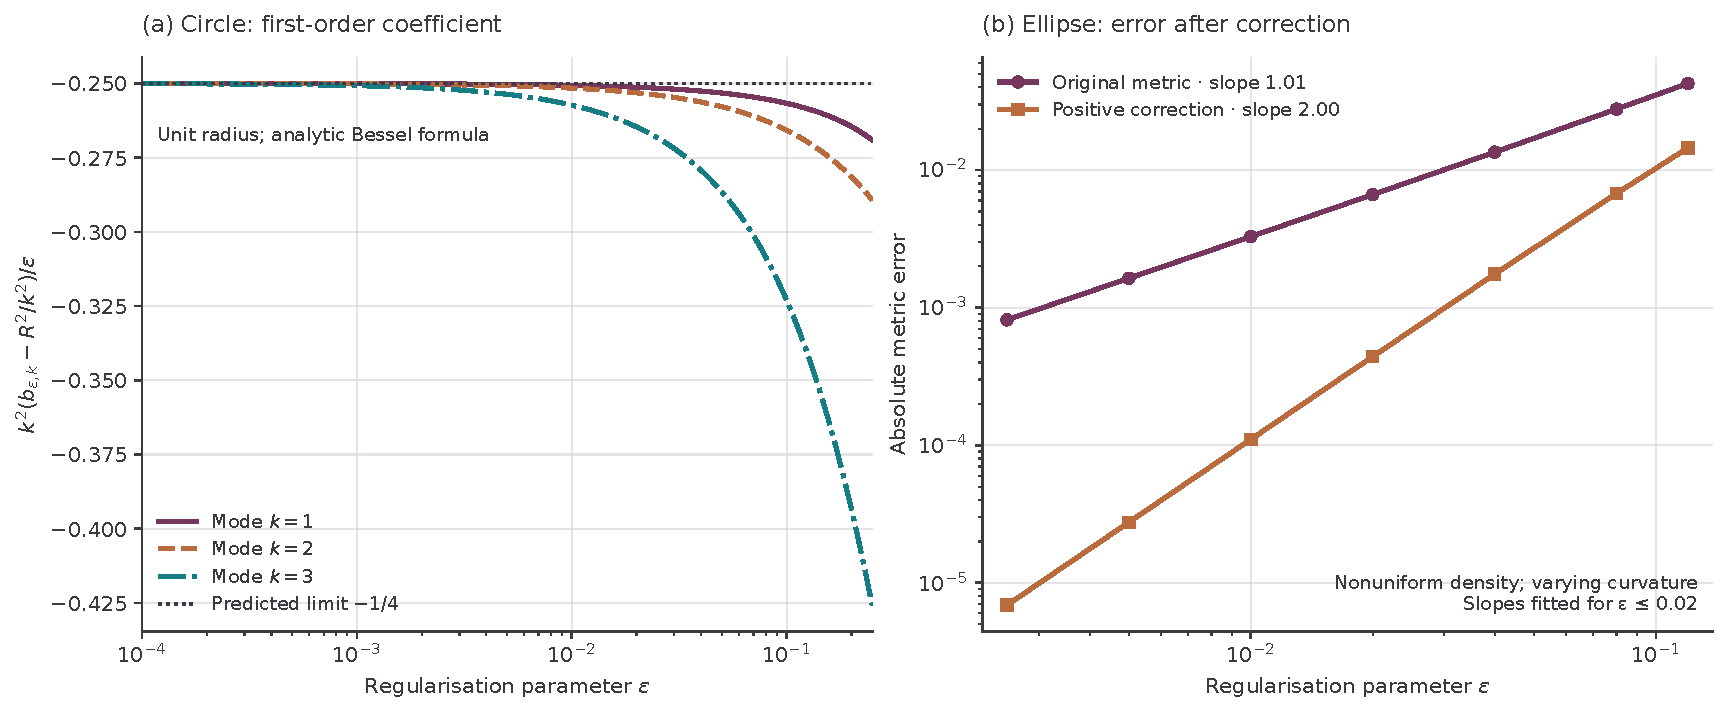
\includegraphics[width=\textwidth]{figures/sinkhorn_curvature_validation.pdf}
\caption{Checks of the fixed-cost expansion. Left: exact circle eigenvalues approach the curvature prediction. Right: the nonuniform ellipse shows first-order raw error and second-order error after the positive correction. All curves concern the stated deterministic examples.}\end{figure}}{}

\section{Embedding dependence, meaning and limits}\label{sec:meaning}

\noindent\emph{This section makes the embedding dependence precise and records what the results do not show.}

The leading Wasserstein tangent metric uses the intrinsic geometry of $M$. The first Sinkhorn bias also uses the second fundamental form of its embedding. Two isometric embeddings can therefore share the same limiting metric and have different finite-regularisation biases. Formula \eqref{eq:bias} makes that dependence explicit. It also explains why a second-order smooth-direction rate proved for a periodic heat kernel cannot automatically be used for a fixed ambient Gaussian cost.

\begin{proposition}[Embedding dependence]\label{prop:embedding}
Let $\iota_1,\iota_2$ be isometric embeddings of the same closed Riemannian manifold $(M,g)$ into Euclidean spaces, with the same density $\rho$, and let $Q_1,Q_2$ be their tensors \eqref{eq:Q}. For smooth centred $h$, with $\phi=A^{-1}h$,
\[
g^{(1)}_{\eps,\mu}(h\mu,h\mu)-g^{(2)}_{\eps,\mu}(h\mu,h\mu)
=-\frac\eps4\int_M\langle(Q_1-Q_2)\nabla\phi,\nabla\phi\rangle\dd\mu+O(\eps^2).
\]
Moreover, for every closed $M\subset\R^D$, $Q$ is positive definite on a nonempty open set $U$ (for example near a point of maximal $|x|$, where $\langle Qv,v\rangle\ge|v|^2/\max_M|x|^2$). Hence the first-order bias $-\tfrac\eps4\int\langle Q\nabla\phi,\nabla\phi\rangle\dd\mu$ is strictly negative whenever $\nabla\phi$ does not vanish identically on $U$, and it vanishes only if $Q\nabla\phi\equiv0$.
\end{proposition}
\begin{proof}
The limit $g_0$ and the operator $A$ depend only on $(M,g,\rho)$, so the first claim is \eqref{eq:bias} applied twice. At a point $x_0$ where $|x|^2$ is maximal, the second derivative of $|x|^2$ along a unit-speed geodesic $\gamma$ with $\dot\gamma=v$ is $2+2\langle x_0,\II(v,v)\rangle\le0$, so $|\II(v,v)|\ge1/|x_0|$ for unit $v$. Taking $e_1=v$ in \eqref{eq:Q}, $\langle Qv,v\rangle\ge|\II(v,v)|^2\ge|x_0|^{-2}$. Thus $Q(x_0)\ge R_{\max}^{-2}I$ with $R_{\max}=|x_0|=\max_M|x|$; by continuity, on a sufficiently small neighbourhood $Q\ge(2R_{\max}^2)^{-1}I$. The final claims follow from $Q\ge0$.
\end{proof}

\paragraph{Examples.} (i) \emph{Curves of equal length.} Every closed curve of length $2\pi$ is isometric to the unit circle. For uniform arclength density and $\phi=\cos s$ the limit is $g_0=1/2$ for every such curve, but the first coefficient is $-\tfrac14\int\kappa(s)^2\sin^2s\,\dd s/2\pi$. For the round circle it is $-1/8$; for the ellipse with semi-axes $1.3$ and $0.6443$ (also of length $2\pi$), with $s$ measured from the end of the major axis, it is $-0.04262$, and a direct Sinkhorn computation gives $-0.04262$ (Richardson). Averaged over rotations of the direction, $\phi=\cos(s-s_0)$, the coefficient becomes $-\tfrac18\int\kappa^2\dd s/2\pi$. For convex plane curves $\int\kappa\dd s=2\pi$, so the Cauchy--Schwarz inequality shows this average is at most $-1/8$, with equality only for the round circle; for the ellipse it is $-0.2059$. The bias of a single direction can therefore be smaller or larger than for the round circle, but the circle minimises the size of the averaged bias. (ii) \emph{Flat tori.} The flat torus $\R^2/(2\pi r_1\mathbb Z\times2\pi r_2\mathbb Z)$ embeds as $\gamma_1\times\gamma_2\subset\R^2\times\R^2$ for any closed curves of lengths $2\pi r_1,2\pi r_2$, with $Q=\operatorname{diag}(\kappa_1^2,\kappa_2^2)$. The round product has $Q=\operatorname{diag}(r_1^{-2},r_2^{-2})$. Products of non-round curves give the same intrinsic metric and a different, non-constant $Q$. No embedding has $Q\equiv0$.

The correction is nonpositive at first order, but the theorem does not claim $g_\eps\leq g_0$ for all $\eps$, all densities or all directions. If the curvature integral vanishes, a higher-order term decides the comparison. The expansion is uniform on fixed smooth families; it need not be uniform for directions whose spatial frequency diverges as $\eps\to0$.

The exact operator limit holds in operator norm on centred $L^2$ at rate $O(\eps^{1/2})$ (Theorem~\ref{thm:rate}); whether the sharp rate $O(\eps)$ holds in general is open. It is not a proof of convergence of unrestricted geodesic distances on the full space of probability measures: minimising paths may leave every compact smooth positive family. Nor does the paper identify ambient squared-distance transport between distant measures with intrinsic Wasserstein transport on $M$. The boundaryless assumption removes boundary layers; positive density removes degeneracy of the weighted elliptic inverse. Domains with boundary, vanishing densities, noncompact tails, and joint empirical-sample/regularisation limits require additional analysis.

\paragraph{Practical notes.} The relative bias is about $\eps/(4R^2)$ for the smallest curvature radius $R$, so it matters only when $\eps$ is not small compared with $4R^2$. Intrinsic costs, such as squared geodesic distance or a heat-kernel cost, do not produce this extrinsic term at first order. The formula in \eqref{eq:corrector} assumes access to the embedding curvature. Estimating that curvature from noisy finite data introduces another error source, which is not included here. The numerical experiments show that the analytic correction can work for controlled smooth examples; they do not establish a general computational advantage.

\section*{Declarations}

\paragraph{Reproducibility.} The accompanying bundle contains the editable manuscript, a formula-first novelty report, Python checks, numerical outputs and figure-generation code. The mathematical results are analytic; no numerical experiment is a premise of a theorem. Literature searches were performed on 1 and 4 November 2026; the novelty report distinguishes inspected full text from abstract-only records.

\paragraph{Use of AI.} AI systems assisted the literature search, derivations, independent checking, code and writing. The author is responsible for the content. The paper has not been externally peer reviewed.

\paragraph{Competing interests and funding.} None.

\paragraph{Archive and licence.} Version 0.1.0-candidate, archived at \url{https://doi.org/10.5281/zenodo.23940148} (all versions: \url{https://doi.org/10.5281/zenodo.23940147}); author Anonymous; text, figures and data CC0-1.0, code MIT.

\begin{thebibliography}{99}
\small\setlength{\itemsep}{3pt}
\bibitem{AtkinsonHan} Atkinson, K., \& Han, W. (2012). \emph{Spherical harmonics and approximations on the unit sphere: An introduction} (Lecture Notes in Mathematics). Springer Berlin Heidelberg. \url{https://doi.org/10.1007/978-3-642-25983-8}
\bibitem{CL} Cheng, X., \& Landa, B. (2024). Bi-stochastically normalized graph Laplacian: Convergence to manifold Laplacian and robustness to outlier noise. \emph{Information and Inference: A Journal of the IMA, 13}(4), iaae026. \url{https://doi.org/10.1093/imaiai/iaae026}
\bibitem{CoifmanLafon} Coifman, R. R., \& Lafon, S. (2006). Diffusion maps. \emph{Applied and Computational Harmonic Analysis, 21}(1), 5--30. \url{https://doi.org/10.1016/j.acha.2006.04.006}
\bibitem{EPglobal} Anonymous. (2026). \emph{Curvature, relative entropy, and global Sinkhorn convergence} (Version 0.1.0-candidate) [Preprint]. Zenodo. \url{https://doi.org/10.5281/zenodo.23929617}
\bibitem{Guo} Guo, H. (2026). \emph{Intrinsic and extrinsic bias of diffusion operators: Asymptotic expansion and kernel-dependent comparison} [Preprint; abstract only inspected, full text not accessible]. SSRN. \url{https://doi.org/10.2139/ssrn.7411565}
\bibitem{HAvL2005} Hein, M., Audibert, J.-Y., \& von Luxburg, U. (2005). From graphs to manifolds -- weak and strong pointwise consistency of graph Laplacians. In \emph{Learning Theory} (Lecture Notes in Computer Science, pp. 470--485). Springer Berlin Heidelberg. \url{https://doi.org/10.1007/11503415_32}
\bibitem{HAvL2007} Hein, M., Audibert, J.-Y., \& von Luxburg, U. (2006). \emph{Graph Laplacians and their convergence on random neighborhood graphs} [Preprint]. arXiv. \url{https://arxiv.org/abs/math/0608522}
\bibitem{Kessler} Kessler, N., Magnet, R., \& Feydy, J. (2025). \emph{Sinkhorn normalization of diffusion kernels} [Preprint]. arXiv. \url{https://arxiv.org/abs/2507.06161}
\bibitem{LLMST} Lavenant, H., Luckhardt, J., Mordant, G., Schmitzer, B., \& Tamanini, L. (2025). The Riemannian geometry of Sinkhorn divergences. \emph{Annales de l'Institut Henri Poincar\'e C, Analyse non lin\'eaire, 43}(5), 1079--1144. \url{https://doi.org/10.4171/AIHPC/165}
\bibitem{LLS} Lavenant, H., Luckhardt, J., \& Schmitzer, B. (2026). \emph{Approximation and computation of the geodesic Sinkhorn distance} [Preprint]. arXiv. \url{https://arxiv.org/abs/2610.02007}
\bibitem{LiYau} Li, P., \& Yau, S. T. (1986). On the parabolic kernel of the Schr\"odinger operator. \emph{Acta Mathematica, 156}, 153--201. \url{https://doi.org/10.1007/BF02399203}
\bibitem{LiouLu} Liou, J.-M., \& Lu, C.-C. (2025). \emph{Asymptotic expansion of the Gaussian integral operators on Riemannian submanifolds of $\R^n$} [Preprint]. arXiv. \url{https://arxiv.org/abs/2506.13238}
\bibitem{MC} Marshall, N. F., \& Coifman, R. R. (2019). Manifold learning with bi-stochastic kernels. \emph{IMA Journal of Applied Mathematics}. \url{https://doi.org/10.1093/imamat/hxy065}
\bibitem{MX} Mordant, G., \& Xu, L. (2026). \emph{Convergence of the Sinkhorn Riemannian metric for finitely supported measures} [Preprint]. arXiv. \url{https://arxiv.org/abs/2609.14651}
\bibitem{DLMF} National Institute of Standards and Technology. (n.d.). \emph{NIST Digital Library of Mathematical Functions}, \S10.32 (Integral representations) and \S10.40 (Asymptotic expansions for large argument). Retrieved November 4, 2026, from \url{https://dlmf.nist.gov/10.32} and \url{https://dlmf.nist.gov/10.40}
\bibitem{Navas} Navas, P. (2026). \emph{The information geometry of the Sinkhorn divergence on a Hilbert manifold} [Preprint]. arXiv. \url{https://arxiv.org/abs/2610.39850}
\bibitem{SchubrBias} Schubr, S. (2026). \emph{Leading bias and positive correction of heat-kernel Sinkhorn metrics} (Edition 2) [Author-posted preprint, not peer reviewed]. Luminary Research Archive. \url{https://research.luminaryoddities.com/leading-bias-positive-correction-heat-kernel-sinkhorn-metrics/v/2}
\bibitem{SchubrSharp} Schubr, S. (2026). \emph{Sharp convergence of heat-kernel Sinkhorn metrics} (Edition 2) [Author-posted preprint, not peer reviewed]. Luminary Research Archive. \url{https://research.luminaryoddities.com/sharp-convergence-of-heat-kernel-sinkhorn-metrics/v/2}
\bibitem{Singer} Singer, A. (2006). From graph to manifold Laplacian: The convergence rate. \emph{Applied and Computational Harmonic Analysis, 21}(1), 128--134. \url{https://doi.org/10.1016/j.acha.2006.03.004}
\bibitem{SWW} Smolyanov, O. G., von Weizs\"acker, H., \& Wittich, O. (2004). \emph{Chernoff's theorem and discrete time approximations of Brownian motion on manifolds} [Preprint]. arXiv. \url{https://arxiv.org/abs/math/0409155}
\bibitem{SEC} Sule, S., Evans, L., \& Cameron, M. (2025). Sharp error estimates for target measure diffusion maps with applications to the committor problem. \emph{Applied and Computational Harmonic Analysis, 79}, 101803. \url{https://doi.org/10.1016/j.acha.2025.101803}. Preprint: \url{https://arxiv.org/abs/2312.14418}
\bibitem{WR} Wormell, C. L., \& Reich, S. (2021). Spectral convergence of diffusion maps: Improved error bounds and an alternative normalization. \emph{SIAM Journal on Numerical Analysis, 59}(3), 1687--1734. \url{https://doi.org/10.1137/20M1344093}
\end{thebibliography}
\end{document}
